% !TEX TS-program = pdflatexmk


\documentclass[11pt]{report}

\usepackage[
%	notes,
	backend=biber,
%	isbn=false,
%	annotation,
%	notetype=endonly
	]{biblatex}
%\DeclareFieldFormat{addendum}{\paragraph\indent{\textbf{Suggestions for Future Research:}\addspace#1}\\}\DeclareFieldFormat{annotation}{\paragraph\indent{\textbf{Brad's Notes:}\addspace#1}\\}
%\DeclareFieldFormat{institution}{\paragraph\indent{\textbf{Institution:}\addspace#1}\\}


\usepackage{tikz}
\usetikzlibrary{arrows}
\usetikzlibrary{shapes}
\usetikzlibrary{patterns}
\usetikzlibrary{positioning}
\usetikzlibrary{decorations.pathmorphing}
%\usetikzlibrary{patterns,positioning,decorations.pathmorphing,arrows,shapes
\usetikzlibrary{fit}

\usepackage{pgfmath}
\usepackage[edges]{forest}

\usepackage{setspace}
\usepackage{amsmath}
\usepackage{amsthm}
	\newtheorem*{theorem}{Theorem}
	\newtheorem*{lemma}{Lemma}
	\newtheorem*{definition}{Definition}
\usepackage{amssymb}

\usepackage{array}
\usepackage{multirow}

\usepackage{hyperref}
\usepackage{url}
\usepackage{enumerate}
\usepackage{enumitem}
\setlist{noitemsep}

\usepackage{listings}
\lstset{language=C}

\usepackage{makeidx}
\usepackage{verbatim}
\usepackage{datetime}
%\usepackage[strings]{underscore}

\setcounter{tocdepth}{2}

\setlength{\pdfpageheight}{11in}
\setlength{\textheight}{9in}
\setlength{\voffset}{-1in}
\setlength{\oddsidemargin}{0pt}
\setlength{\marginparsep}{0pt}
\setlength{\marginparwidth}{0pt}
\setlength{\marginparpush}{0pt}
\setlength{\textwidth}{6.5in}

\def\sinline[#1]{ \ \tikz\draw[decorate,decoration={snake,amplitude=0.6mm, segment length=14pt},->] (0,0) -- (.6,0) node [midway, above] {#1}; \ }

\pagestyle{plain}
\makeindex

\title{Prospectus Report:  Imbalanced Data}
\author{Brad Burkman}
\newdateformat{vardate}{\THEDAY\ \monthname[\THEMONTH]\ \THEYEAR}
\vardate
\date{Updated \today}

\addbibresource{../../../Summer_2021/619/Accident_Analysis_and_Prevention/Accident_Analysis_and_Prevention.bib}

\addbibresource{../../../Spring_2022/699/Papers/BibFile_Spring_2022.bib}

\addbibresource{../../../Summer_2021/619/Transportation_Research_Part_C/Transportation_Research_Part_C.bib}

\addbibresource{../../../Fall_2021/699/Bib_Files/Old_Files/Ambulance.bib}

\addbibresource{../Papers/TRpC_vol_098_140.bib}

\addbibresource{../Papers/AAP_vol_122_173.bib}

\addbibresource{../Papers/Medium_TDS_Citations.bib}


% Tell BiBTeX to ignore the abstract.  
\DeclareSourcemap{
  \maps[datatype=bibtex]{
    \map{
      \step[fieldset=abstract, null]
    }
  }
}


\begin{document}
\setlength{\parindent}{20pt}
\begin{spacing}{1.2}
\setcounter{chapter}{-1}


\maketitle
\tableofcontents

%%%%%%%%%%%%%%%%%%
% Index
% Example of how to put something in the index:
% This item will be listed as "Definition" under the heading of "Articulation Node."
%		\index{Articulation Node!Definition}

\newpage
\phantomsection
\addcontentsline{toc}{chapter}{Index}
\printindex


%%%%%%%%%%
\chapter{To Do}

%%%%%
\section{Topics Remaining}

\subsection{Big Items}

\begin{itemize}
	\item Crash Analysis Lit Review
	\item Data Overview and Analysis
	\item Research Plan
\end{itemize}

\subsection{Details}
\begin{itemize}
	\item Worked through Brad's Reports
	\item Find where it mentions multiple Tomek runs.  
	\item Work through this tutorial, which will explain Condensed Nearest Neighbor.
	
	https://machinelearningmastery.com/undersampling-algorithms-for-imbalanced-classification/
	
	\item Figure out what Rough Sets Theory and Fuzzy Sets are.  
	\item Learn to use ROC curves.
	\item Review different types of models and how to implement them in Keras.
	\item Bagging and Boosting
	\item Topological Data Analysis
	
	Giotto-tda is a Python package dedicated to integrating TDA in the machine learning workflow by means of a scikit-learn API

\end{itemize}

%%%%
\section{Plan}

\begin{itemize}
	\item Identify review papers by established experts that give overviews of the field.  Use these as a ``textbook'' for imbalanced data.
	\item Write a review of the field (similar to my study guide for the Algorithms Comp)
	\begin{itemize}
		\item Topics
		\begin{itemize}
			\item Benchmark datasets for imbalanced classification.
			\item Sampling methods
			\item Metrics
			\item Loss functions
			\item Bagging and Boosting
			\item Math and CS tools, like Principal Component Analysis
		\end{itemize}
		\item For each topic
		\begin{itemize}
			\item Original and significant papers
			\item Theory and rationale
			\item Examples of usage in the field
			\item Example where I implement it
			\item If appropriate, implement it on the crash data
		\end{itemize}

	\end{itemize}
\end{itemize}

%%%%%
\section{Paper Standards}

When I took a 619 with Dr. Raghavan, he rejected my first draft of my paper because it could be summarized as, ``I used existing methods to do the same thing other people have done, but on my own data.''  He expected me to have done more thinking and synthesis.  

I had written the paper that way because that's what most of the papers I'd read did.  I learned later that I had been reading in a low-ranked journal.  

I feel like most of the {\it Accident Analysis and Prevention} papers are like that, ``I did a thing!''  If this field had benchmark datasets, it would be easier to see what is actually new in each article.  The {\it AAP} journal is not well ranked.  The {\it Transportation Research: Part C, Emerging Technologies} is better in both content and rankings.  I'll use the {\it TRC} articles as models.

%%%%%
\section{Paper Outline Idea from 7/19/21 Report}

\begin{enumerate}
	\item Louisiana Crash Dataset and its Challenges
	\begin{enumerate}[label=\alph*.]
		\item General Description
		\item Some data is missing
		\item Some data is unreliable or obviously wrong
		\item Data is imbalanced
	\end{enumerate}
	\item Incorporating Other Data
	\begin{enumerate}[label=\alph*.]
		\item Weather
		\item Urban/Rural
	\end{enumerate}
	
	\item Data Cleanup:  Methods
	\begin{enumerate}[label=\alph*.]
		\item Comparison of methods for handling missing data
		\item Methods for dealing with outliers
	\end{enumerate}
	\item Features:  Methods
	\begin{enumerate}[label=\alph*.]
		\item Engineering New Features
		\item Selecting Features [Incorporate Jing Chen's methods]
	\end{enumerate}
	\item Imbalanced Data:  Comparison of Methods
	\begin{enumerate}[label=\alph*.]
		\item Oversampling
		\item Understampling
		\item \verb|class_weight = 'balanced'|
		\item Finding balance between methods [pun intended]
	\end{enumerate}
	\item New Metrics: {\it Balanced Precision} and {\it Balanced f1}
	\begin{enumerate}[label=\alph*.]
		\item Definitions
		\item Justification
		\item Examples
	\end{enumerate}
	\item Models
	\item Balancing Everything
	\item Conclusion
	
\end{enumerate}
 



%%%%%%%%%%
\chapter{Introduction}
%%%%%
\section{Problem}

%%%
\subsection{Application}

\index{Google Pixel Phone}
\index{iPhone}
\index{GM OnStar}

New (starting in 2022) Google Pixel phones have a feature that will automatically alert the police when involved in an automobile crash.  Apple says the feature is coming to iPhones \index{iPhone} and Apple Watches soon; those products already have a feature that detects a person falling, calls the person, and if no response, calls a neighbor, a friend, or the police.  One of my friends with multiple sclerosis uses this app.

Such systems (like GM OnStar) \index{GM OnStar}, built into vehicles, have existed for years, but soon they will become ubiquitous.  When the police receive a notification, based on the information they have, should they automatically deploy an ambulance?  In an accident with severe (but not instantly fatal) injuries, a few minutes' delay may have serious consequences, but sending an ambulance is expensive, and their supply is limited.  Can we develop a model that will, from the limited information the police can hope to have, from the datasets we have chosen, build a model to make a good prediction of whether an ambulance is needed?  

I am using ``police'' as a shorthand for ``the decision makers at the emergency call center.''  

This new cell phone feature will not be perfect; it will give many false positives and may not detect crashes with small objects, like pedestrians, \index{Pedestrian} that do not cause severe deceleration but are most likely to have severe injury.  The automated reports may, however, give us additional information like the number of people (number of phones) involved, and speed at time of impact.  This new phone feature will keep the crash analysis community busy for many years.  

The ``make a good predicition'' part is complicated.  We are not going to get 100\% accuracy.   What would we mean by ``good,'' and what would we use as a basis of comparison?  The current system relies mostly on phone calls from eyewitnesses who can give more information than the police will have in an automated notification.  These are thorny questions that we must address.  

%%%
\subsection{Datasets}

I am looking at two datasets,  the US \acrfull{dot} \acrfull{nhtsb} \acrfull{crss} data 2016-2020 data ($\approx 250,000$ records), and a census of Louisiana crash records 2014-18 ($\approx 800,000$ records).

%%%
\subsection{Imbalanced Data}
\index{Imbalanced Data}

In the 2014-2018 Louisiana data, we have over eight hundred thousand crash records.  If we are just looking for fatal crashes, about 3500 were fatal, 0.42\%.  If we built a model to predict whether a crash is fatal, and the model predicted that all crashes were nonfatal, that model would have correctly classified 99.58\% of crashes, or have 99.58\% {\it accuracy}.  In most contexts, that level of accuracy would be amazing, but in this context, such a model would be useless. 

In the CRSS dataset, which over represents severe crashes, 81.15\% of people involved in a crash were not transported to the hospital, and 16.75\% went to the hospital (the remaining 2.10\% unknown).  This nearly 5:1 imbalance is not as severe as the example with fatalities above, but still will be a challenge for our usual model building algorithms to give us the insights we want.  

The problem of imbalanced data appears in many applications, including spam detection and credit card fraud detection, and over the last fifty years the community has built many tools for addressing the problem.  Using those tools is as much art as science, and the best combination of methods depends on the dataset and desired outcome.  The desired outcome is a moral, ethical, and political question as well as a technical one.  

%The dataset classifies the crashes as ``Fatal,'' ``Severe,'' ``Moderate,'' ``Complaint,'' and ``No Injury,'' also called PDO, ``Property Damage Only.''  Note that ``Fatal'' does not mean that everyone involved died, so there may be people moderately or seriously injured who need urgent medical attention.  If we are looking to model whether a crash is Fatal or Severe, those together are 1.1\%, and Fatal/Severe/Moderate is 6.8\%.  

%%%
\subsection{Tradeoffs}

Balancing false positives and false negatives in this application is additionally problematic because they have different costs.  The cost of a false positive (sending an ambulance when one is not needed) is measured in dollars, but the cost of a false negative (not sending an ambulance when one is needed) is measured in lives.  It is likely that this study will only illustrate the choices to be made rather than find a Goldilocks solution that will significantly increase the number of true positives without increasing the number of false positives.  



%%%%%
\section{Novel Contributions of this Work (Knowledge Gap)}

Novel Aspects of this Work

\begin{itemize}
	\item New Real-World Problem:  Newly emerging problem of how to use the greatly increasing volume of automated crash notification data.
	\item New Dataset:  The Louisiana dataset has not appeared significantly in the literature.
	\item New Imputation of Unknown Values in Well Known Dataset
	\item New Metrics:  Balanced Precision and Balanced F1
	\item Interpretation of Class Weights as a Political/Ethical Cost-Benefit Tradeoff
	\item New Combinations of Methods:  The Louisiana data is very incomplete, dirty, and imbalanced, and the CRSS data is imbalanced.  Off-the-shelf methods will not give the level of confidence needed for life-and-death decisions.  
\end{itemize}

%%%%%%%%%%
\chapter{Lit Review:  Crash Analysis}

%%%%%
\section{Journals}

\noindent\begin{tabular}{@{}p{4in}p{1in}p{1in}}
	Journal & CiteScore & Impact Factor \cr\hline
	\it Accident Analysis and Prevention & 7.8 & 4.993 \cr
\end{tabular}

\begin{quote}
Accident Analysis \& Prevention provides wide coverage of the general areas relating to accidental injury and damage, including the pre-injury and immediate post-injury phases. Published papers deal with medical, legal, economic, educational, behavioral, theoretical or empirical aspects of transportation accidents, as well as with accidents at other sites. Selected topics within the scope of the Journal may include: studies of human, environmental and vehicular factors influencing the occurrence, type and severity of accidents and injury; the design, implementation and evaluation of countermeasures; biomechanics of impact and human tolerance limits to injury; modelling and statistical analysis of accident data; policy, planning and decision-making in safety. 
\end{quote}

\noindent\begin{tabular}{@{}p{4in}p{1in}p{1in}}
	\it American Journal of Emergency Medicine & 3.2 & 2.469 \cr
\end{tabular}

	\begin{quote}
	A distinctive blend of practicality and scholarliness makes the American Journal of Emergency Medicine a key source for information on emergency medical care. Covering all activities concerned with emergency medicine, it is the journal to turn to for information to help increase the ability to understand, recognize and treat emergency conditions. Issues contain clinical articles, case reports, review articles, editorials, international notes, book reviews and more. The American Journal of Emergency Medicine is recommended for initial purchase in the Brandon-Hill study, Selected List of Books and Journals for the Small Medical Library (2001 Edition).
	\end{quote}

\noindent\begin{tabular}{@{}p{4in}p{1in}p{1in}}
	\it Decision Support Systems & 10.5 & 5.795 \cr
\end{tabular}

	\begin{quote}	
	The common thread of articles published in Decision Support Systems is their relevance to theoretical and technical issues in the support of enhanced decision making. The areas addressed may include foundations, functionality, interfaces, implementation, impacts, and evaluation of decision support systems (DSSs). Manuscripts may draw from diverse methods and methodologies, including those from decision theory, economics, econometrics, statistics, computer supported cooperative work, data base management, linguistics, management science, mathematical modeling, operations management, cognitive science, psychology, user interface management, and others. However, a manuscript focused on direct contributions to any of these related areas should be submitted to an outlet appropriate to the specific area.

Examples of research topics that would be appropriate for Decision Support Systems include the following:

1. DSS Foundations e.g. principles, concepts, and theories of enhanced decision making; formal languages and research methods enabling improvements in decision making. It is important that theory validation be carefully addressed.

2. DSS Functionality e.g. methods, tools, and techniques for developing thefunctional aspects of enhanced decision making; solver, model, and/or data management in DSSs; rule formulation and management in DSSs; DSS development and use in computer supported cooperative work, negotiation, research and product.

3. DSS Interfaces e.g. methods, tools, and techniques for designing and developing DSS interfaces; development, management, and presentation of knowledge in a DSS; coordination of a DSS's interface with its functionality.

4. DSS Implementation - experiences in DSS development and utilization; DSS management and updating; DSS instruction/training. A critical consideration must be how specific experiences provide more general implications.

5. DSS Evaluation and Impact e.g. evaluation metrics and processes; DSS impact on decision makers, organizational processes and performance.
	\end{quote}

\noindent\begin{tabular}{@{}p{4in}p{1in}p{1in}}
	\it Journal of Safety Research & 5.0 & 3.487 \cr
\end{tabular}

	\begin{quote}	
The Journal of Safety Research is a multidisciplinary publication that provides for the exchange of scientific evidence in all areas of safety and health, including traffic, workplace, home, and community. While this research forum invites submissions using rigorous methodologies in all related areas, it focuses on basic and applied research in unintentional injury and illness prevention. Affiliated with the National Safety Council, it seeks to engage the global scientific community including academic researchers, engineers, government agencies, policy makers, corporate decision makers, safety professionals and practitioners, psychologists, social scientists, and public health professionals.
	\end{quote}

\noindent\begin{tabular}{@{}p{4in}p{1in}p{1in}}
	\it Transportation Research Part C:  Emerging Technologies & 14.0 & 8.089 \cr
\end{tabular}

	\begin{quote}	
The focus of Transportation Research: Part C (TR\_C) is high-quality, scholarly research that addresses development, applications, and implications, in the field of transportation systems and emerging technologies . The interest is not in the individual technologies per se, but in their ultimate implications for the planning, design, operation, control, maintenance and rehabilitation of transportation systems, services and components. In other words, the intellectual core of the journal is on the transportation side, not on the technology side. The integration of quantitative methods from fields such as operations research, control systems, complex networks, computer science, artificial intelligence are encouraged.

Of particular interest are the impacts of emerging technologies on transportation system performance, in terms of monitoring, efficiency, safety, reliability, resource consumption and the environment. Submissions in the following areas of transportation are welcome: multimodal and intermodal transportation; on-demand transport; intelligent transportation systems; traffic and demand management; real-time operations; connected and autonomous vehicles; logistics; railways; resource and infrastructure management; aviation; pedestrians and soft modes.

Special emphasis is given in open science initiatives and promoting the opening of large-scale datasets for papers published in TR\_C that can support transferability and benchmarking of different approaches. The realization of data opportunities that arise from emerging technologies and new sensors in transportation can revolutionize how this data reshape our understanding of congestion mechanisms and can contribute in efficient and sustainable mobility management.	
	\end{quote}


%%%%%
\section{Articles using Similar Datasets}

\begin{itemize}
	\item Rahim 2021 \cite{RAHIM2021106090} LSU faculty, similar dataset to what we have.  
	\item Jiang 2020 \cite{JIANG2020105520} used similar data and addressed the challenges we'll have with it.  
	
\end{itemize}

%%%%%
\section{Articles on Imbalanced Crash Data}

\begin{itemize}
	\item  Schlogl 2020 \cite{SCHLOGL2020105398} uses imbalanced data.
\end{itemize}

%%%%%
\section{Ambulances}

%%%
\subsection{Ambulance Response Time}

From 11/29/21 Report.

\begin{itemize}
	\item Found standard for emergency medical service (EMS) response time, from The National Fire Protection Association.
	``1710 NFPA Standard for the Organization and Deployment of Fire Suppression Operations, Emergency Medical Operations,  and Special Operations to the Public by Career Fire Departments, 2020''
	  \S 4.1.2.1
	\begin{itemize}
		\item 60-second turnout time 
		\item 240  seconds  or  less  travel  time  for  the  arrival  of  a  unit with  first  responder  with  automatic  external  defibrillator (AED) or higher-level capability at an emergency medical incident
		\item 480 seconds or less travel time for the arrival of an advanced  life  support  (ALS)  unit  at  an  emergency  medical  incident,  where  this  service  is  provided  by  the  fire department  provided  a  first  responder  with  an  AED  or basic  life  support  (BLS)  unit  arrived  in  240  seconds  or less travel time.
		\item Lots of papers, like Liu (2016)\cite{Liu_2016} cite Rafael Sa'adah (2004), which I think is a response to the NFPA standards, but I can't find it online or in the library database.
	\end{itemize}	
\end{itemize}

%%%%%
\section{iPhone to Automatically Detect Crash and Call Emergency Services}

From 11/29/21 Report.

\begin{itemize}
	\item iPhones and Apple Watches will soon automatically call police when the accelerometer detects a car crash.
	\item Several articles dated 11/1/21, including in the Wall Street Journal.  
	\item Available in 2022
	\item What data would that provide, and what data would the police already have to complement it?  These are just my guesses.
	\item Data from Apple
	\begin{itemize}
		\item Registered owner of the phone (or phones) in the car
		\item Typical users of that phone (Apple knows!)
		\item GPS location
		\item Perhaps a rough idea of how fast the car was going and how suddenly it stopped
		\item If more than one phone sends signal, do these people know each other, or are they likely in different vehicles?
		\item Accelerometer signature of a pedestrian or bicyclist getting hit?
	\end{itemize}
	\item Complementary data from police database
	\begin{itemize}
		\item Type of roadway and speed limit
		\item Was it at an intersection?
		\item Time of day, day of week
		\item Type of vehicle registered to that person
		\item Driving record of user of phone (History of DUI?)
		\item Weather
	\end{itemize}
\end{itemize}

%%%%%
\section{Weather}

From 11/29/21 Report.

\begin{itemize}
	\item Wang et al \cite{WANG2020102619} studied the data of a ride-hailing company, DiDi Chuxing, and looked for how resilient the system was during ``extreme weather events.''  
	\begin{itemize}
	\item They defined such weather to be ``hurricane, flooding, and rainstorm.'' (page 2)   I suspect that ``rainstorm,'' which is really vague in English, is a poor translation of a more specific Chinese word.  
	\item Because these extreme events are rare, they have a sample imbalance problem (page 13).  They solve the problem in an interesting way, by ignoring it and watering down their data set.  ``The characteristics of urban transportation resilience under catastrophic events have generally similar patterns to those under general precipitation events.  Thus we incorporated the rainstorm and usual prediction events data into [sic] data set to strengthen the model training.''  So, as I understand it, they had an imbalanced data problem modeling extreme weather, so they just modeled ordinary weather.  
	\item I like how the authors started their methodology section with a page of definitions.  
	\end{itemize}
	
\end{itemize}


%%%%%
\section{Lagniappe}

\begin{itemize}
	\item Osman 2019 (LSU) \cite{OSMAN2019274} looked much more deeply at the data than other studies, looking for correlations between sets of variables.  
	\item Ziakopoulos 2020 \cite{ZIAKOPOULOS2020105323} is a good overview of the field and its jargon.  
	
	\item Guimmarra 2020 \cite{GIUMMARRA2020105333} is interesting for its text mining of crash reports.  

	\item Park 2019 \cite{Park_2019} has a full-page table categorizing studies of ambulance location, relocation, and dispatching using different optimization methods.  

\end{itemize}


%%%%%
\section{Significant Authors}

From 11/15/21 Notes:

Reviewed all of the 66 articles from 2021 with the word ``crash''  in {\it Transportation Research Part C:  Emerging Technologies}. 

\begin{itemize}
	\item Most of the articles are about autonomous vehicles.
	\item Mohammed Abdel-Aty at the U of Central Florida is a major author in this journal, but not in this year.  In previous years, if there was an article from UCF, his name was on it.  His website does not say that he has retired.  
	\item When I write, I want to include more examples than many authors give.  
\end{itemize}

%%%%%
\section{TR\_C Articles on Machine Learning}

\subsection{Application of articles whose keywords contain {\it machine learning}, {\it deep learning}, or {\it reinforcement learing}}

\begin{itemize}
	\item Autonomous Vehicles
	\begin{itemize}

	\item Control of Autonomous Vehicles 
		\cite{AN2020102777},
		\cite{BAUTISTAMONTESANO2022103662},
		\cite{CAO2022103656},
		\cite{DONG2021103192},
		\cite{DU2022103489}, 
		\cite{GUO2021102980},
		\cite{KALATIAN2021102962},
		\cite{LAZAR2021103258},
		\cite{LI2022103452},
		\cite{SHI2021103421}, 
		\cite{WANG2022103478},
		\cite{WEGENER2021102967},
		\cite{WU2020102649},
		\cite{YE2019155}, 
		\cite{ZHANG2021103140}, 
		\cite{ZHU2020102662},
	\item Preferences for Autonomous Vehicles
		\cite{ZHANG2020102774}
	\end{itemize}
		
% Lagniappe
	\item Lagniappe
	\begin{itemize}		
	\item Anomalous Event Prediction
		\cite{YANG2021102862},
	\item Origin/Destination
		\cite{MA2020102747},
		\cite{SUN2021103114},
		
	\item Variable Speed Limits 
		\cite{WU2020102649}
		
	\item Dynamic Pricing 
		\cite{GENSER2022103485},
		\cite{HAN2022103584},
		\cite{PANDEY2020102715}
	\item Parking
		\cite{MANTOUKA2021103173},
		\cite{YANG2019248},
		\cite{ZHANG2022103624}
	\item Traffic Signal Optimization 
		\cite{LEE2019117},
		\cite{LI2021103059}, 
		\cite{WANG2021103046},
		\cite{WANG2022103670},
		\cite{WU2019246},
		\cite{YOON2021103321},
	\item Perimeter Metering (?) 
		\cite{ZHOU2021102949}
	\item Energy Consumption
		\cite{QI201967},
		\cite{YAO2019276}
	\item Vehicle Idenfification
		\cite{DABIRI2020102644},
		\cite{LI2021102946},
	\item Trip Purpose
		\cite{FAROQI2021103131}
	\end{itemize}
	
% Traffic		
	\item Traffic
	\begin{itemize}
	\item Traffic Prediction
		\cite{BACHIR2019254},
		\cite{BOGAERTS202062},
		\cite{CUI2020102620},
		\cite{DAI2019142},
		\cite{DO201912},
		\cite{DRCHAL2019370},
		\cite{KUMAR2021103432},
		\cite{LI2021102977},
		\cite{LI2021103185},
		\cite{LI2021103389},
		\cite{MA2020352},
		\cite{ROY2021103339},
		\cite{WANG2020102763},
		\cite{WONG2020247},
		\cite{YANG2021103228},
		\cite{ZHANG2021103372},
		\cite{ZHANG2022103659},
	\item Traffic Speed Prediction 
		\cite{NAIR2020269},
		\cite{REMPE2022103448},
		\cite{WANG2019372},
		\cite{ZHANG2019297}
	\item Traffic in Extreme Weather
		\cite{WANG2020102619}
	\item Traffic Signals
		\cite{GUO2021103416},
		\cite{MAHMOUD2021102930},
		\cite{ZHAO2022103522}
	\item Dynamic Traffic Control  
		\cite{SHOU2022103560}
	\end{itemize}

% Individual Driver
	\item Individual Driver
	\begin{itemize}
	\item Vehicle Behavior Modeling
		\cite{CHEN2020102646},
		\cite{MA2020102785},
		\cite{MO2021103240}, 
		\cite{RAHMAN2021103310},
		\cite{YAO2021103415},
		\cite{ZHANG2019287}
	\item Classifying Driving Styles 
		\cite{MOHAMMADNAZAR2021102917}
	\item Driver's Visual Environment
		\cite{CAI2022103541},
		\cite{LI2019132},
		\cite{MA2019317}
	\item Driver Behavior
		\cite{MOHAMMADNAZAR2021102917},
		\cite{XING2021103288},
	\item Driver Distraction 
		\cite{CAI2022103541}
	This article is interesting, perhaps relevant to me, for correlating crashes with something else.

	\end{itemize}
	
% Delivery
	\item Delivery
	\begin{itemize}
	\item Delivery Times
		\cite{HUGHES2019289},
	\item Vehicle Routing Problem
		\cite{XU2022103620},
		\cite{ZHANG2020102861}
	\item Fleet Management
		\cite{TURAN2020102829}
	
	\item Transportation Systems [Survey article] 
		\cite{WANG2019144}
	\end{itemize}
	
% Public Transit
	\item {Public Transit}
	\begin{itemize}
	\item Taxis
		\cite{CHEN2021103272},
		\cite{JIAO2021103289},
		\cite{KE2021102858},
		\cite{MAO2020102626}, 
		\cite{QIN2021103239},
		\cite{SHOU2020102738}, 
		\cite{TANG2020102844},
		\cite{YU2022103640},
	\item Public Transit
		\cite{CHOW2021103264},
		\cite{FENG2022103611},
		\cite{LIU201918},
		\cite{MULLERHANNEMANN2022103566},
		\cite{TANG2021102951},
		\cite{WANG2019387},
		\cite{WANG2020102661},
		\cite{ZHANG2021102928}
	\end{itemize}

% Pedestrians and Passengers
	\item Pedestrians and Passengers
	\begin{itemize}
	\item Pedestrians
		\cite{BUSTOS2021103018},
		\cite{HIDAKA2019115}
	\item Bicycles and Scooters
		\cite{ITO2021103371},
		\cite{LV2021103404},
		\cite{ZUNIGAGARCIA2022103660},
	\item Travel Demand Modeling
		\cite{HAFEZI2021102972},
		\cite{KIM2022103523},
		\cite{LI2021102921},
		\cite{LIU2021103361},
		\cite{PANG2020102706}
	\end{itemize}

% Planes and Trains
	\item {Planes, Trains, and Boats}
	\begin{itemize}
	\item Railway Maintenance
		\cite{ALLAHBUKHSH201935}
	\item Railway Traffic Control
		\cite{GHASEMPOUR202091},
		\cite{TANG2022103679}
	\item Train Delays
		\cite{LI2022103606},
		\cite{NAIR2019196}
	\item Air Traffic Management 
		\cite{BAO2021103323},
		\cite{ALBABA2021103417},
		\cite{CORRADO2021103331},
		\cite{DESHMUKH2021103036},
		\cite{DHIEF2022103704},
		\cite{DU2021103122},
		\cite{KHAN2021103225},
		\cite{OLIVE2020102737},
		\cite{PANG2021103326},
		\cite{PHAM2022103463},
		\cite{SCHULTZ2021103119},
		\cite{VERDONKGALLEGO2019356},
		\cite{WANG2021102892},
		\cite{ZHU2021103179},
	\item Ships
		\cite{GUMUSKAYA2021103383},
		\cite{LU2021102970},
	\end{itemize}
	
% Crashes
	\item Crashes
	\begin{itemize}
	\item Inferring Pre-Crash Impact Data
		\cite{CHEN2021103009},
	\end{itemize}
	
% Back End
	\item Back End (No Application)
	\begin{itemize}
	\item Generative Modeling
		\cite{BORYSOV201973},
		\cite{GARRIDO2020102787}
	\item Preference Learning
		\cite{ZHU2020102849}
	\item Extracting Economic Information (?)
		\cite{WANG2020102701}
	\item Graphs
		\cite{RODRIGUEZDENIZ2022103556}
	\item Discrete Choice Models
		\cite{SFEIR2022103552}
	\item Fairness in Artificial Intelligence
		\cite{ZHENG2021103410}
	\item Discrete Choice Modeling
		\cite{WONG2021103050}
	\end{itemize}

\end{itemize}
 
\subsection{Articles whose abstracts refer to imbalanced data}

\vskip 0pt

Chen \cite{CHEN2020102646} talks about resampling using SMOTE and Tomek.  Used LightGBM classifier.  

Cai \cite{CAI2020102697} used the deep convolutional generative adversarial network (DCGAN).  Compared four models, logistic regression model, support vector machine, artificial neural network, and convolutional neural network.  

Emarani Abou Elassad \cite{ELAMRANIABOUELASSAD2020102708} works with several imbalanced methods.  Use this paper as a model.  

Yu \cite{YU2020102740} used focal loss for real-time crash prediction.  

Shi \cite{SHI2021103414} uses the Grey Wolf Optimizer and SMOTE to balance the data.  

Khan \cite{KHAN2021103225} used SMOTE and ``average balanced recall accuracies,''

Chen \cite{CHEN2022103709} uses bagging.

Anomalous events might also use imbalanced data.  

\subsection{Crashes}

Twenty-one articles in TR\_C have 'crash', 'accident', 'ambulance', 'hospital', 'fatal', or 'injury' in the keywords.  Another forty have them in the abstract.  I'm really only interested in ones that use real data, not simulation.  

Kalatian \cite{KALATIAN2021102962} studies interactions between pedestrians and autonomous vehicles.  

Cai and Abdel-Aty \cite{CAI2020102697} do similar work to ours with machine learning.

Emarani Abou Elassad \cite{ELAMRANIABOUELASSAD2020102708} was mentioned above as a model paper.  Also applied to crashes.  

Yu \cite{YU2020102740} mentioned above.  











%%%%%%%%%%
\chapter{Lit Review:  Data Cleaning}

%%%%%
\section{Cleaning Techniques Used in Crash Analysis Studies}


In ``A deep learning based traffic crash severity prediction framework'' by Rahim (LSU) \cite{RAHIM2021106090}, they just deleted any records with missing or inconsistent data.  The {\it Titanic} Kaggle sites you showed me use several other methods for filling in incomplete data.  Write a paper where I compare different methods for dealing with missing data, and their effect on different metrics (precision, recall, accuracy, sensitivity, f1, false alarm rate) of the classification of the test set.  

Rahim's article took out 37\% of the records for missing or inconsistent data, but only 21\% of the fatal crashes; could that imbalance in the data cleaning skew the model prediction?  It makes sense that police would be more meticulous in their record keeping for fatal crashes, but 21\% and 37\% are huge.  

Would we get a better model if we found a good way to fill in missing data?



%%%%%%%%%%
\chapter{Lit Review: Methods for Imbalanced Data}

%%%%%
\section{Algorithm Level Approaches}
\index{Algorithm Level Approaches}

%%%
\subsection{Some Papers}
\begin{itemize}
	\item Recognition-based:  Learning from one class rather than discrimination-based, doing unsupervised learning on the minority class. \cite{CHAWLA_2004}
	\item Fuzzy rule-based classification systems (what is this?)
		\cite{CHABBOUH_2019} 
		\cite{DABLAIN_2021}
		\cite{MAHMUDAH_2021} 
		\cite{ZHAI_2020} 
		\cite{ZHAI_2020_D2GAN}
	\item In decision trees, using evolutionary/genetic methods instead of greedy search 
		\cite{CHABBOUH_2019} 
		\cite{WEISS_2000}
	\item Clustering and Subspace Modeling \cite{CHEN_2011}
\end{itemize}

%%%
\subsection{Genetic Algorithms}
\index{Genetic Algorithms}

In this short 2000 paper, Weiss \cite{WEISS_2000} used a genetic algorithm to predict rare events. Borrowing from simulated annealing, they varied the relative importance of precision and recall at each step of the genetic algorithm.  

%%%
\subsection{Subspace Model}
\index{Subspace Model}

Chen 2011 \cite{CHEN_2011}

This was fascinating and entirely different from anything I've seen.  

\begin{enumerate}
	\item Separate the training data $Tr$ into negative (majority) and positive (minority) classes $TrN$ and $TrP$.
	\item Let $K$ be the ratio of negative to positive samples, in my case about 100, so that if you divide the majority class $TrN$ into $K$ groups, each will have about the same number of samples as the minority class.
	\item Use $K$-means clustering to separate the negative (majority) class $TrN$ into $K$ groups; each of the groups is a cluster of the negative (majority) class.
	\item For each of the $K$ groups $TrN_i$:
	\begin{itemize}
		\item Combine the negative elements of the group with the entire positive (minority) class $TrP$ to form a balanced subspace.  
		\item Train the model for the subspace
	\end{itemize}
	\item Recombine the $K$ subspace models with a model trained on the entire data set to build an integrated model.
\end{enumerate}


%%%%%
\section{Metrics}

%%%
\subsection{The Problem:  Imbalanced Data Set}

In an unbalanced data set, the number of actual negatives ($N = TN + FP$) is much different from the number of actual positives ($P = FN + TP$).  In our case, if our independent variable is fatal crashes, the negatives are $99.574714\%$ of the data set, and the positives are just $0.425286\%$.

The standard metrics get thrown off by the imbalance.  If we predict that every crash is nonfatal, we have accuracy of 99.57\%, which sounds really impressive.  

The recall (true positive rate) is not thrown off by an imbalanced data set, because it only works with TP and FN, the actual positives.  Similarly for specificity (true negative rate).

The precision is thrown off by an imbalanced data set, because it works with both a subset of the actual positives (TP) and a subset of the actual negatives (FP).  


%%%
\subsection{Standard Metrics}

\hfil \begin{tabular}{cc|c|c|}
	&\multicolumn{1}{c}{}& \multicolumn{2}{c}{Prediction} \cr
	&\multicolumn{1}{c}{} & \multicolumn{1}{c}{N} & \multicolumn{1}{c}{P} \cr\cline{3-4}
	\multirow{2}{*}{Actual}&N & TN & FP \cr\cline{3-4}
	&P & FN & TP \cr\cline{3-4}
\end{tabular}

\begin{align*}
	\text{Accuracy} &= \frac{TN+TP}{TN+FP+FN+TP} \cr
	\text{Recall or TPR} &= \frac{TP}{TP + FN} \cr
	\text{Specificity, Selectivity, or TNR} &= \frac{TN}{TN + FP} \cr
	\text{Precision} & = \frac{TP}{TP + FP}\cr
\end{align*}

%%%
\subsection{Balanced Precision and Balanced f1 in the Penalty Function}

Most ML algorithms work using a {\it penalty function} that measures how bad the current solution is, then iteratively improving the solution in the direction that minimizes the penalty.  We should be able to write a custom penalty function.  

\

Update:  How-to instructions for changing the metrics in {\tt scikit-learn}.  The example is how to use recall instead of accuracy.  

\url{https://stackoverflow.com/questions/54267745}


\

{\it Recall} only deals with the minority class, so the balance of the data set doesn't matter.  {\it Precision}, on the other hand, takes results from both classes, so we can balance it by scaling the count of False Positive results, giving a {\it Balanced Precision} metric.  From Recall and Balanced Precision we can get a {\it Balanced f1} metric.  

If our penalty function uses balanced precision and balanced f1, it may not matter that our data set is imbalanced, and we can use all of, and only, the original data to build our model.  

%%%
\subsection{Balanced Precision in the Literature}

{\it Balanced Accuracy} frequently appears in the literature.  I have not found {\it balanced precision} in the literature.  Two possible reasons.  Either nobody has thought of it, or they did, found it not useful, and abandoned the idea.

\

Update:  {\tt imbalanced-learn} has more metrics than {\it scikit-learn}, but still no balanced precision.  

\url{https://imbalanced-learn.org/dev/metrics.html}



%%%
\subsection{Balanced Accuracy}

There is a metric called {\it balanced accuracy}.  You get it from the definition of {\it accuracy} by multiplying the actual negative elements (TN and FP) by the ratio of the positives to negatives, 

$$\frac{P}{N} = \frac{FN+TP}{TN+FP}$$

so that the total number of actual negatives and total number of actual positives in the sample are equal.

[I suppose you could also get it by multiplying the actual positive elements (FN and TP) by the reciprocal.]

I got this derivation by intuiting about what I would want {\it balanced accuracy} to mean, and it matches the definition I found in Wikipedia.  

\url{https://en.wikipedia.org/wiki/precision_and_recall#Imbalanced_data}

Wikipedia says [I'm sure I can find a more authoritative source.]

$$\text{Balanced Accuracy} = \frac{TPR + TNR}{2}$$

\begin{align*}
	\text{Recall or TPR} &= \frac{TP}{TP+FN} \cr
	\text{Specificity or TNR} &= \frac{TN}{TN+FP} \cr
	\text{Accuracy} &= \frac{TN+TP}{TN+FP+FN+TP} \cr
	\text{Balanced Accuracy} &=  \frac{TN \cdot \frac{P}{N}+TP}{TN \cdot \frac{P}{N}+FP \cdot \frac{P}{N}+FN+TP} \cr
		&= \frac{TN \cdot P+TP \cdot N}{TN \cdot P+FP \cdot P+FN \cdot N+TP\cdot N} \cr
	&= \frac{TN \cdot P+TP \cdot N}{(TN+FP) \cdot P+(FN+TP) \cdot  N} \cr
	&= \frac{TN (FN+TP)+TP (TN+FP)}{(TN+FP) (FN+TP)+(FN+TP) (TN+FP)} \cr
	&= \frac{TN (FN+TP)+TP (TN+FP)}{2(TN+FP) (FN+TP)} \cr
	&= \frac{TN (FN+TP)}{2(TN+FP) (FN+TP)}  + \frac{TP (TN+FP)}{2(TN+FP) (FN+TP)} \cr
	&= \frac{TN}{2(TN+FP) }  + \frac{TP }{2 (FN+TP)} \cr
	&= \frac{TNR+TPR}{2} \cr
\end{align*}

%%%
\subsection{Balanced Precision}

I haven't found {\it balanced precision} in a brief Google search, although Google knows the kind of stuff I look up and sent me to articles on balanced accuracy.  Finding it will take some work, because ``balanced precision'' has different meanings in other tech fields.  

We can make balanced precision the same way we made balanced accuracy, by taking the actual negative results (TN and FP) and scaling them  so that the total number of actual negatives equals the total number of actual positives, by multiplying by $\frac{P}{N} = \frac{FN+TP}{TN+FP}$.

Is this related to the G-mean?  [No]

$$\text{G-mean} = \sqrt{\text{Precision} \times \text{Specificity}}$$

\begin{align*}
	\text{Precision} &= \frac{TP}{TP+FP} \cr
	\text{Balanced Precision} &= \frac{TP}{TP+FP \cdot \frac{P}{N}} \cr
		&= \frac{TP \cdot N}{TP \cdot N + FP \cdot P} \cr
		&= \frac{TP (TN+FP)}{TP(TN+FP) + FP (FN+TP)} \cr
		&= \frac{TP (TN+FP)}{TP(TN+FP) + FP (FN+TP)} \cr
		&= \dots \cr
\end{align*}

Giving up here on finding some nice, concise connection between Balanced Precision and other metrics.  


%%%
\subsection{Balancing Two Metrics:  F1 and Gmean}

From Elassad 2020:
\cite{ELAMRANIABOUELASSAD2020102708}

\begin{quote}
F1 score, is a highly informative measure as it considers both precision and recall measures, which makes it very suitable for
imbalanced classification (Qian et al., 2014; Sun et al., 2018); it’s deemed to be a special measure that conveys the balance between
the precision and recall in order to find an effective and efficient trade-off. Another useful metric is G-mean, which is considered as a
metric of stability between correct classification of positive class and negative class viewed independently. It is usually adopted in
order to resist the imbalances in the dataset (Kubat et al., 1997).
\end{quote}


\subsubsection{F1 Metric}
\index{F1}

F1 is the harmonic mean of Precision and Recall.  

$$\text{F1} = \frac{2}{\frac{1}{\text{Precision}} + \frac{1}{\text{Recall}}} 
	= \frac{2 \cdot TP}{2\cdot TP + FP + FN}$$

%%%
\subsubsection{Gmean}
\index{Gmean}

Gmean is the geometric mean of Precision and Specificity (TNR).

\begin{align*}
	\text{Precision} & = \frac{TP}{TP + FP}\cr
	\text{Specificity, Selectivity, or TNR} &= \frac{TN}{TN + FP} \cr
	\text{Gmean} &= \sqrt{ \text{Precision} \times \text{Specificity}} \cr
	&= \sqrt{
		\frac{TP}{TP+FP} \times \frac{TN}{TN+FP}
		}
\end{align*}







%%%%%
\section{Loss Functions}

%%%%%
\subsection{Binary Cross-Entropy Loss Function}
\index{Binary Cross-Entropy}

Let's say we have an imbalanced data set with 100 negative samples for each positive sample.  

For binary classification, the first three (class weights, weighted loss function, and na\"{i}ve oversampling) are effectively the same in the training phase.  The cross-entropy loss function, 

$$loss = \sum_{i=1}^n y_i \log(p_i) + (1-y_i) \log (1-p_i)$$

for binary classification is

$$loss = \sum_{y_i=1} \log (p_i) + \sum_{y_i=0} \log (1-p_i)$$

which is the sum of the logs of the errors in predictions for the negative class plus the sum of the logs of the errors in predictions for the positive class.  

%%%
\subsection{Class Weights and $\alpha$-weighted Loss}
\index{Class Weights}
\index{$\alpha$-Weighted Loss}

If the classes are imbalanced, like there are 100 times as many samples with $y=0$ as samples with $y=1$, then the loss function is mostly summing how bad the predicting probability is for the majority class and largely ignoring the minority class.  Both the class weights parameter and a weighted loss function fix this by multiplying one or the other by some compensating factor.

$$loss = 100 \times \sum_{y_i=1} \log (p_i) +  \sum_{y_i=0} \log (1-p_i)$$

This multiple gives the two classes equal weight in the loss.  

In the $\alpha$-weighted cross entropy, 

$$loss = \sum_{i=1}^n \alpha y_i \log(p_i) + (1 - \alpha) (1-y_i) \log (1 - p_i)$$

let $\alpha = \frac{100}{100+1}$ and you'll get the same thing, within a positive constant multiple.  

$$loss = \sum_{i=1}^n \frac{100}{101} y_i \log(p_i) + \frac{1}{101} (1-y_i) \log (1 - p_i)$$

$$loss = \frac{1}{101}\sum_{i=1}^n 100 y_i \log(p_i) + (1-y_i) \log (1 - p_i)$$

The only difference I can ascertain between the class weights parameter and a weighted loss function is that the class weights aren't used with the validation set.  

%%%
\subsection{Oversampling}
\subsection{Na\"{i}ve Oversampling}
\index{Oversampling (Random)}

Na\"{i}ve oversampling would be to create 99 copies of each of the positive samples, so that the two sets are balanced.  That would have exactly the same effect on the loss function, because there would now be 100 times as many samples with $y_i=1$.  

%%%%%
\subsection{Class Weights v/s Na\"{i}ve Oversampling: They're the Same}

I had an insight on why these things are the same.  Let's say you have an imbalanced data set, with 100 times as many negative samples as positive samples.  

In Na\"{i}ve Oversampling, you make 100 copies of each of the positive samples and run regular cross-entropy loss.  

In weighted Class Entropy, you multiply the positive-class losses by 100.

$$loss = 100 \times \sum_{y_i=1} \log (p_i) +  \sum_{y_i=0} \log (1-p_i)$$

These two approaches different in execution but the same in result because, as I often remind my students, multiplying something by 100 is the same as adding it to itself 100 times.  



%%%
\subsection{Focal Loss}
\index{Focal Loss}

Introduced by Lin in 2017.  \cite{LIN_2020}

Yu 2020 \cite{YU_2020} adapts $\alpha$-weighted cross entropy and focal loss to crash analysis.


In the focal loss function, 

\begin{align*}
	loss &= \sum_{i=1}^n \alpha (1 - p_i) ^{\gamma_1} y_i \log (p_i) + (1 - \alpha) p_i^{\gamma_2} (1 - y_i)  \log (1 - p_i) \cr
	loss &= \sum_{y_i=1} \alpha (1 - p_i) ^{\gamma_1} \log (p_i) + \sum_{y_i=0} (1 - \alpha) p_i^{\gamma_2}   \log (1 - p_i) \cr
	\end{align*}

if $\gamma_1= \gamma_2 = 0$, then it's the same as the $\alpha$-weighted loss function.  

In the original focal loss paper by Lin \cite{LIN_2020}, $\gamma_1$ and $\gamma_2$ are the same.  

For samples with $y_i=1$, the minority class, here are values of $(1 - p_i) ^{\gamma_1} \log (p_i)$ for different values of $p_i$ and different values of $\gamma_1$.  I got the range of values of $\gamma_1 \in \{0, 0.5, 1, 2, 5\}$ from Lin's 2018 paper  that proposed focal loss.  

\begin{center}
\begin{tabular}{rl | llllll}
	&& \multicolumn{5}{c}{$\gamma_1$} \cr
	$(1 - p_i) ^{\gamma_1} \log (p_i)$ & & 0 & 0.5 & 1 & 2 & 5 \cr \hline
	& 0.1 & -3.32 & -3.15 & -2.99 & -2.69 & -1.96 \cr
	& 0.3 & -1.74 & -1.45 & -1.22 & -0.85 & -0.29 \cr
	$p_i$ & 0.5 & -1 & -0.71 & -0.5 & -0.25 & -0.03 \cr
	& 0.7 & -0.51 & -0.28 & -0.15 & -0.05 & 0 \cr
	& 0.9 & -0.15 & -0.05 & -0.02 & 0 & 0 \cr\end{tabular}
\end{center}

If $\gamma_1 > 0$, then for samples in the positive class, the loss is negligible for good predictions ($p_i$ close to 1), so it focuses the loss on poor predictions.  

Yu applied focal loss in the crash literature.\cite{YU_2020}

%%%
\subsection{Optimizing $F_\beta$}
\index{$F_\beta$}

Loss functions for gradient-based learning need to be differentiable (?), and the $F_\beta$ score is not differentiable, so this 2021 article by Lee \cite{LEE_2021} proposes a differentiable surrogate loss function that optimizes the $F_\beta$ score.  

With imbalanced data, using a loss function that optimized $F_\beta$ instead of accuracy would let you balance precision and recall, fixing one aspect of the imbalance problem.  

$$F_\beta = \frac{(1+\beta^2) \cdot \text{Precision} \cdot \text{Recall}}{(\beta^2 \cdot \text{Precision}) + \text{Recall}} 
= \frac{1}{
	\displaystyle\frac{\lambda_\beta}{\text{Recall}} + \frac{1 - \lambda_\beta}{\text{Precision}}
	}, 
	\qquad
	\lambda_\beta = \frac{\beta^2}{1 + \beta^2}
$$

The article takes a deep dive into loss functions.  I should master it.  


%%%
\subsection{Tree-Based Methods}
\index{Tree-Based Methods}


Pendault \cite{PEDNAULT_2000} has a 2000 article on insurance risk modeling that incorporates ``a domain-specific optimization criterion... to identify suitable splits during tree building.''  It assigns different weights to {\it claim} and {\it nonclaim} records.  Because that strategy helps but does not entirely solve the imbalanced data problem, they also have a split criterion that prevents splits of really small branches, ``splinter groups,'' that are unlikely to contain any elements of the minority class because the minority class is so sparse.  


%%%%%
\subsection{$\alpha$-weighted Binary Cross-Entropy Loss Function as Ethical Tradeoff}
\index{Ethical Tradeoff}
\label{sec:Ethical_Tradeoff}

From \verb|Brads_Report_10_25_21|

I made a [perhaps paper-worthy?] connection between the loss function I want and the $\alpha$-weighted binary cross-entropy loss function, which is widely known and widely implemented, but, according to Yu's paper, not before used in crash-related modeling.  

\subsubsection{Matrix}

\hfil\begin{tabular}{r|c|c|c|}
	& Do Not &  \cr
	& Send & Send \cr
	& Ambulance & Ambulance \cr
	& $h_\theta(x_i)<0.5$ & $h_\theta(x_i)>0.5$  \cr\hline
	Do Not Need Ambulance \  $y_i=0$ & TN & FP \cr \hline
	Need Ambulance \   $y_i=1$ & FN & TP \cr\hline
\end{tabular}

\subsubsection{Switching between Binary and Continuous}

In the binary cross-entropy loss function, 

$$J = -\sum_{i=1}^N y_i \log( h_\theta (x_i)) + (1-y_i) \log( 1 - h_\theta (x_i))$$

the $y_i$ are binary, $y_i \in \{0,1\}$, but the model predictions, $h_\theta (x_i)$, are a probability, $h_\theta(x_i) \in (0,1)$.  


\

If we treat the model predictions as binary, replacing 

$$
\log ( h_\theta(x_i)) \to 
\begin{cases}
	0 & \text{if } h_\theta(x_i) <= 0.5 \cr
	1 & \text{if } h_\theta(x_i) > 0.5 \cr
\end{cases}
$$

and

$$
\log ( 1 -  h_\theta(x_i)) \to 
\begin{cases}
	0 & \text{if } 1 - h_\theta(x_i) <= 0.5 \cr
	1 & \text{if } 1 - h_\theta(x_i) > 0.5 \cr
\end{cases}
$$

then 

$$ TP = \sum_{i=1}^N y_i \log( h_\theta (x_i))$$

$$ TN = \sum_{i=1}^N  (1-y_i) \log( 1 - h_\theta (x_i))$$

and the loss function becomes $J = -(TP+TN)$

Why do we use the continuous instead of the binary in the loss function?  Because we want the predictions to be robust, so that when we use the model on unseen data, we can be more certain that it will correctly classify new instances.  The binary, however, are much easier to explain to non-technical people, or even technical people in other fields.  

%%%
\subsubsection{Scenario}

The medical ethicists and politicians decide on a number, $p$, such that we are willing to automatically dispatch $p$ ambulances when they aren't needed in order to send one ambulance when it is needed.   We want $$ \frac{\Delta FP}{\Delta TP} \le p$$

%%%
\subsubsection{Binary $h_\theta$}

Our loss function is $$FP - p\cdot TP $$

%%%
\subsubsection{Continuous $h_\theta$}

Use the $\alpha$-weighted cross-entropy loss function, as in Yu's paper and widely available.

$$J = -\sum_{i=1}^N \alpha y_i \log( h_\theta (x_i)) + (1-\alpha)(1-y_i) \log( 1 - h_\theta (x_i)), \quad \alpha = \frac{p}{p+1}$$

%%%
\subsubsection{Why are these equivalent?}

Adding a constant to the loss function, or multiplying it by a positive constant, does not change its effect.  

$FP - p \cdot TP$ is equivalent to $FP - p \cdot TP + (TN+FP)$, because $TN+FP$ is constant, so 
$FP - p \cdot TP$ is equivalent to $-(p \cdot TP+ TP)$.


$$FP - p \cdot TP$$
$$-(p \cdot TP + TN)$$
Multiplying by $\frac{1}{p+1}$ gives an equivalent loss function, because $\frac{1}{p+1}>0$.
$$-\frac{p \cdot TP + TN}{p+1}$$
$$- \left( \frac{p}{p+1} TP + \frac{1}{p+1} TN\right)$$
$$- \left( \frac{p}{p+1} TP + \left( 1 - \frac{p}{p+1} \right) TN \right)$$
$$- (\alpha TP + (1 - \alpha) TN) $$

The continuous version of $TP$ is 
$ \displaystyle \sum_{i=1}^N y_i \log( h_\theta (x_i))$

The continuous version of $TN$ is 
$ \displaystyle \sum_{i=1}^N (1-y_i) \log( 1 - h_\theta (x_i))$

$$J = -\sum_{i=1}^N \alpha y_i \log( h_\theta (x_i)) + (1-\alpha)(1-y_i) \log( 1 - h_\theta (x_i)), \quad \alpha = \frac{p}{p+1}$$

%%%
\subsubsection{Emphasis in Our Work}

Yu et al introduced to the crash-analysis field the alpha-weighted cross-entropy loss function to deal with imbalanced data.  We propose another application of the alpha-weighted loss, to encode and implement tradeoffs that come from our ethical/political values decided by community leaders.   



%%%%%
\section{Data Level Methods}
\index{Data Level Methods}

Consider this two-dimensional training dataset, which we will use to illustrate data-level techniques for handling imbalanced datasets.  In real problems, of course, the dataset could have a hundred dimensions and a million samples.  The six blue circles represent samples (elements) of the majority negative class (``no ambulance''), and the three red squares represent the minority positive class (``ambulance'').  


\begin{center}
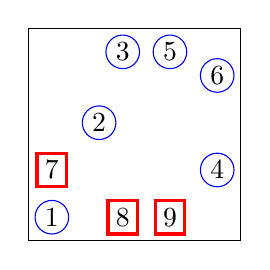
\begin{tikzpicture}[x = 3mm, y=3mm]
	\draw (-1,-1) rectangle (8,8);
	\tikzstyle{Square} = [
		draw = red, 
		very thick,
		rectangle,
		inner sep = 1mm,
		minimum size = 2 mm
	]
	\tikzstyle{SquareFill} = [
		draw = red, 
		fill = red,
		very thick,
		rectangle,
	]
	\tikzstyle{Circle} = [
		draw = blue, 
		circle,		
		inner sep = 0.5mm,
	]
	\tikzstyle{CircleFill} = [
		draw = blue,
		fill = blue, 
		circle,
	]
	\node [Circle] (1) at (0,0) {1};
	\node [Circle] (2) at (2,4) {2};
	\node [Circle] (3) at (3,7) {3};
	\node [Circle] (4) at (7,2) {4};
	\node [Circle] (5) at (5,7) {5};
	\node [Circle] (6) at (7,6) {6};
	\node [Square] (7) at (0,2) {7};
	\node [Square] (8) at (3,0) {8};
	\node [Square] (9) at (5,0) {9};

\end{tikzpicture}
\end{center}

Many algorithms, and variations thereon, have been proposed to balance the two classes before applying a machine learning algorithm to build a model to classify new samples as positive or negative.  WARNING:  Vast oversimplification ahead.  Our goal here is to give the general idea of each method.  


%%%
\subsection{Imbalanced Cleaning:  Tomek and Condensed Nearest Neighbor}
\index{Tomek Links}
\index{Condensed Nearest Neighbor}

Batista
\cite{BATISTA_2004}
uses two imbalanced cleaning method called {\it Tomek links} and {\it Condensed Nearest Neighbor}.  If examples from the majority and minority class are close to each other, it deletes the majority samples.   One could think of it as targeted undersampling of the majority set.  

Imbalanced-Learn, an add-on to Scikit-Learn, has these algorithms read to use.  Tomek and Wilson's papers introducing these algorithms are from the 1970's.  
\index{Imbalanced-Learn}


%%%
\subsection{Tomek's Links}

In 1976, Tomek proposed a method of undersampling that assumes that the majority and minority classes should (at least locally) be clustered. \cite{ivan1976two} If an sample $A$ of the majority class and a sample $B$ of the minority class are each other's nearest neighbors, then one of them is not clustered with its own class.  Since we are trying to undersample the majority class, assume that the element of the majority class is noise (or an error, or just not useful), and delete it.  

In the diagram below, samples \#1 and \#7 are Tomek links, because they are each other's nearest neighbors and of different classes.  Samples \#4 and \#9 are not Tomek links, because while 9 is 4's nearest neighbor, 9's nearest neighbor is 8, not 4.  

In the context of modeling crash severity from police reports, why would sample \#1 not need an ambulance when its characteristics are so close to those of \#7 and not near most of the other crashes without serious injury?  The reason could be errors in the records, or luck/providence/fate.  It could also be that the difference between property damage only and serious injury is influenced by thousands of variables we cannot measure or know, all of the physics of crash forces acting on the bones and structures of the human body.  The best we can say is that the outcome in \#1 cannot be predicted by the information that we have, so that sample will not help in constructing a model based on the available data; therefore, we can reasonably delete it from the training set.  

Tomek's Links can also be run iteratively.  Sample \#7 had \#1 as its nearest neighbor, but once \#1 is deleted, then \#2 and \#7 are each other's nearest neighbors of different classes, thus are Tomek links, and we can delete \#2.  



\begin{center}
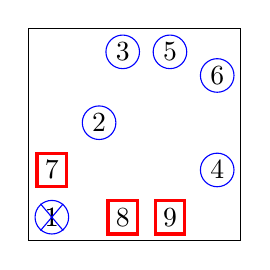
\begin{tikzpicture}[x = 3mm, y=3mm]
	\draw (-1,-1) rectangle (8,8);
	\tikzstyle{Square} = [
		draw = red, 
		very thick,
		rectangle,
		inner sep = 1mm,
		minimum size = 3 mm
	]
	\tikzstyle{SquareFill} = [
		draw = red, 
		fill = red,
		very thick,
		rectangle,
	]
	\tikzstyle{Circle} = [
		draw = blue, 
		circle,
		inner sep = 0.5 mm
	]
	\tikzstyle{CircleFill} = [
		draw = blue,
		fill = blue, 
		circle,
	]
	\node [Circle] (1) at (0,0) {1};
	\node [Circle] (2) at (2,4) {2};
	\node [Circle] (3) at (3,7) {3};
	\node [Circle] (4) at (7,2) {4};
	\node [Circle] (5) at (5,7) {5};
	\node [Circle] (6) at (7,6) {6};
	\node [Square] (7) at (0,2) {7};
	\node [Square] (8) at (3,0) {8};
	\node [Square] (9) at (5,0) {9};

	\node [Circle, cross out] (1) at (0,0) {1};
\end{tikzpicture}
\end{center}

%%% Original stuff in Prospectus

This method undersamples the majority-class samples, eliminating ones that are too close to minority-class samples, presuming them to be noise, and helping clarify clusters of minority samples.  

A pair of samples are a {\it Tomek link} if one is majority and one minority, and they are each other's nearest neighbors. To use Tomek's inks as an undersampling strategy for imbalanced data, delete the positive sample in each Tomek's link.  Other cleaning strategies (for balanced sets) would eliminate both the positive and negative.  

It is possible to iterate Tomek's several times.  Here's an example of how it works in one round and in a second round.  The blue samples are from the majority set and the red are from the minority.  Assume that these seven points are a small part of a large dataset, but these are the only points in this region.

\

\noindent\hfil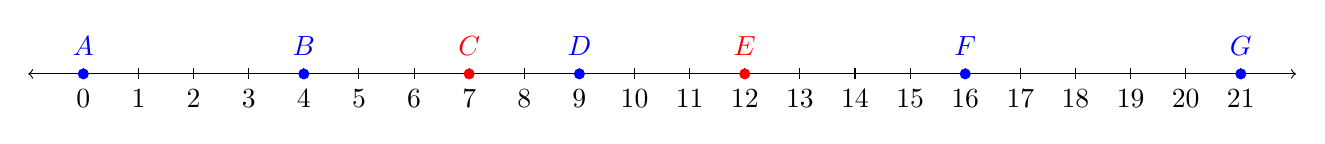
\begin{tikzpicture}[x=7mm, y=7mm]
	\draw [<->] (-1,0) -- (22,0);
	\foreach \x in {0,1,2,...,21}
		\draw (\x, 0.1) -- (\x,-0.1) node [below] {$\x$};
	\fill [blue] (0,0) circle (2pt) node [above=3pt, blue] {$A$};
	\fill [blue] (4,0) circle (2pt) node [above=3pt, blue] {$B$};
	\fill [blue] (9,0) circle (2pt) node [above=3pt, blue] {$D$};
	\fill [blue] (16,0) circle (2pt) node [above=3pt, blue] {$F$};
	\fill [blue] (21,0) circle (2pt) node [above=3pt, blue] {$G$};
	\fill [red] (7,0) circle (2pt) node [above=3pt, red] {$C$};
	\fill [red] (12,0) circle (2pt) node [above=3pt, red] {$E$};
\end{tikzpicture}

In the original dataset, $C$ and $D$ are each other's nearest neighbors, $C$ from minority and $D$ from majority, so they are a Tomek link.   On the other hand, $D$ is the nearest neighbor to $E$, but $E$ is not $D$'s nearest neighbor, so they are not a Tomek link.  

Eliminate sample $D$.  

\

\noindent\hfil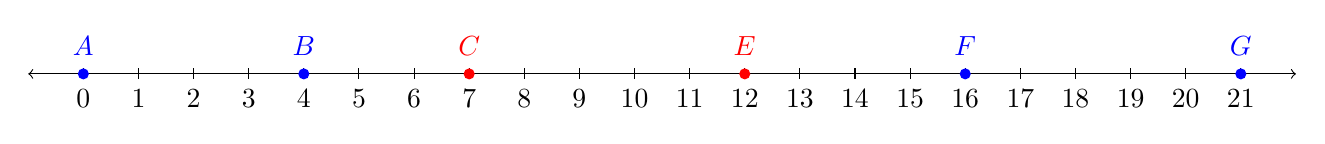
\begin{tikzpicture}[x=7mm, y=7mm]
	\draw [<->] (-1,0) -- (22,0);
	\foreach \x in {0,1,2,...,21}
		\draw (\x, 0.1) -- (\x,-0.1) node [below] {$\x$};
	\fill [blue] (0,0) circle (2pt) node [above=3pt, blue] {$A$};
	\fill [blue] (4,0) circle (2pt) node [above=3pt, blue] {$B$};
%	\fill [blue] (9,0) circle (2pt) node [above=3pt, blue] {$D$};
	\fill [blue] (16,0) circle (2pt) node [above=3pt, blue] {$F$};
	\fill [blue] (21,0) circle (2pt) node [above=3pt, blue] {$G$};
	\fill [red] (7,0) circle (2pt) node [above=3pt, red] {$C$};
	\fill [red] (12,0) circle (2pt) node [above=3pt, red] {$E$};
\end{tikzpicture}

Now the pairs $(B,C)$ and $(E,F)$ are Tomek links, so if we ran Tomek undersampling a second time, we would remove samples $B$ and $F$.  

\

\noindent\hfil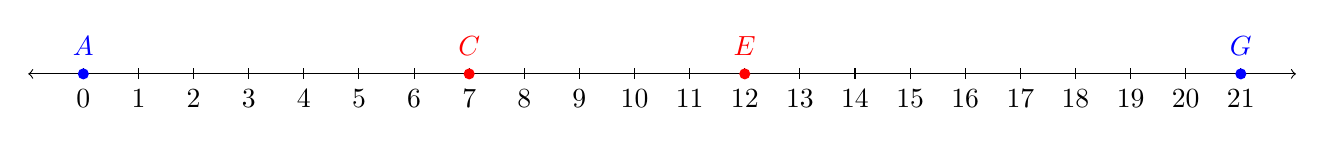
\begin{tikzpicture}[x=7mm, y=7mm]
	\draw [<->] (-1,0) -- (22,0);
	\foreach \x in {0,1,2,...,21}
		\draw (\x, 0.1) -- (\x,-0.1) node [below] {$\x$};
	\fill [blue] (0,0) circle (2pt) node [above=3pt, blue] {$A$};
%	\fill [blue] (4,0) circle (2pt) node [above=3pt, blue] {$B$};
%	\fill [blue] (9,0) circle (2pt) node [above=3pt, blue] {$D$};
%	\fill [blue] (16,0) circle (2pt) node [above=3pt, blue] {$F$};
	\fill [blue] (21,0) circle (2pt) node [above=3pt, blue] {$G$};
	\fill [red] (7,0) circle (2pt) node [above=3pt, red] {$C$};
	\fill [red] (12,0) circle (2pt) node [above=3pt, red] {$E$};
\end{tikzpicture}

Now $C$ and $E$ are each other's nearest neighbors and of the same (minority) class, so this part of the dataset would not change under another run of Tomek.  

The idea of Tomek assumes that the minority samples should cluster, and any majority samples in or near those clusters must be noise, so we can eliminate them.  We now have a clear cluster of two minority samples with no close majority samples.  

I saw multiple runs of Tomek mentioned [somewhere] in my reading, so  I tried it on the crash data, running it up to five times, and saw that it converged, with fewer positive samples eliminated in each round.  I had conjectured that a negative sample in a Tomek link in a later round must have been a negative sample in a Tomek link in an earlier round, digging itself out of a field of positive-class dust, but I suspected that there might be (perhaps unusual) cases where one minority-class sample ($C$ in the example above) created a Tomek link, and eliminating the majority-class sample in that link ($D$ above) allowed a Tomek link for a different minority-class sample ($E$ above).  I then played with it until I found a counterexample to my conjecture, so the conjecture, that a minority-class sample in a Tomek link in a later round of Tomek undersampling must have been in a Tomek link in every previous round of the Tomek undersampling, is false.  

If the conjecture had been true, then we could greatly speed up subsequent rounds of Tomek undersampling by only considering the minority samples in Tomek links in the previous round.  That would not be thorough, but this approach would.  

\subsubsection{Algorithm for Repeated Application of Tomek's Links}

	For the first round of Tomek undersampling, one has to consider each element of the minority class.  In the Tomek's links, call the minority-class elements $\{A_{1}, A_{2}, \dots, A_{n1}\}$, and the majority-class elements $\{B_1, B_2, \dots, B_{n1}\}$.  Tomek undersampling for minority classes eliminates all of $\{B_1, B_2, \dots, B_{n1}\}$.
	
	In the second round of Tomek undersampling, we only need to consider as possible Tomek links the nearest neighbors of $\{A_{1}, A_{2}, \dots, A_{n1}\}$ and any element of the minority class that had one of $\{B_1, B_2, \dots, B_{n1}\}$ as its nearest neighbor.
	
In subsequent rounds, consider the minority-class samples from the Tomek's links from the previous round, and the elements of the minority class that had as their nearest neighbor an element of the majority class in the Tomek's links.  

In theory there could be more Tomek's links in one round than in the previous round, but in practice they go to zero and the set converges to a set with no Tomek's links.  

%%%
\subsection{Cleaning Multiclass Data}
\index{Cleaning Multiclass Data}

Wei (2021) \cite{WEI_2021} uses something similar to Tomek's links for a multi-class problem with a majority class and multiple minority classes.  

\begin{itemize}
	\item Splits an imbalanced multi-class problem with $n+1$ classes ($n$ of them being minority) into $n$ imbalanced binary problems for data cleaning.  
	\item Uses cleaning undersampling (similar to Tomek's Links) to remove noisy spots in the data.
\end{itemize}


%%%
\subsection{Random Oversampling}
\index{Oversampling (Random)}

Random (na\"{i}ve) oversampling creates duplicates of minority class samples until the sets are balanced.  This method has a similar effect to using class weights, introduced below.  

\begin{center}
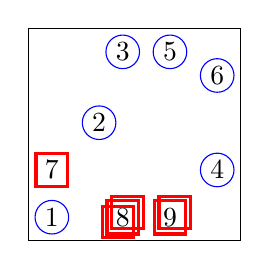
\begin{tikzpicture}[x = 3mm, y=3mm]
	\draw (-1,-1) rectangle (8,8);
	\tikzstyle{Square} = [
		draw = red, 
		very thick,
		rectangle,
		inner sep = 1mm,
		minimum size = 4 mm
	]
	\tikzstyle{SquareFill} = [
		draw = red, 
		fill = red,`	
		very thick,
		rectangle,
	]
	\tikzstyle{Circle} = [
		draw = blue, 
		circle,
		inner sep = 0.5 mm
	]
	\tikzstyle{CircleFill} = [
		draw = blue,
		fill = blue, 
		circle,
	]
	\node [Circle] (1) at (0,0) {1};
	\node [Circle] (2) at (2,4) {2};
	\node [Circle] (3) at (3,7) {3};
	\node [Circle] (4) at (7,2) {4};
	\node [Circle] (5) at (5,7) {5};
	\node [Circle] (6) at (7,6) {6};
	\node [Square] (7) at (0,2) {7};
	\node [Square] (8) at (3,0) {8};
	\node [Square] (9) at (5,0) {9};

%	\node [Square] (7) at ($(0,2) + (-0.2,-0.2)$) {};
	\node [Square] (8) at ($(3,0) + (-0.2,-0.2)$) {};
%	\node [Square] (9) at ($(5,0) + (-0.2,-0.2)$) {};

%	\node [Square] (7) at ($(0,2) + (0.2,0.2)$) {};
	\node [Square] (8) at ($(3,0) + (0.2,0.2)$) {};
	\node [Square] (9) at ($(5,0) + (0.2,0.2)$) {};


\end{tikzpicture}
\end{center}

Na\"{i}ve oversampling would be to create 99 copies of each of the positive samples, so that the two sets are balanced.  That would have exactly the same effect on the loss function, because there would now be 100 times as many samples with $y_i=1$.  


%%%
\subsection{Undersampling}
\index{Undersampling (Random)}

Random undersampling balances the two classes by randomly deleting elements of the majority class until the two are balanced.  The major drawback of this method is that you throw away information about the majority class.  If the majority class is many more times the size of the minority, you lose almost all of the data.  


\begin{center}
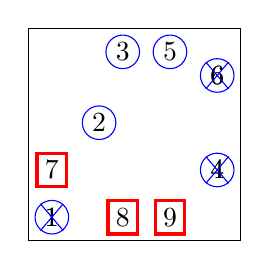
\begin{tikzpicture}[x = 3mm, y=3mm]
	\draw (-1,-1) rectangle (8,8);
	\tikzstyle{Square} = [
		draw = red, 
		very thick,
		rectangle,
		inner sep = 1 mm,
		minimum size = 3 mm
	]
	\tikzstyle{SquareFill} = [
		draw = red, 
		fill = red,
		very thick,
		rectangle,
	]
	\tikzstyle{Circle} = [
		draw = blue, 
		circle,
		inner sep = 0.5 mm
	]
	\tikzstyle{CircleFill} = [
		draw = blue,
		fill = blue, 
		circle,
	]
	\node [Circle] (1) at (0,0) {1};
	\node [Circle] (2) at (2,4) {2};
	\node [Circle] (3) at (3,7) {3};
	\node [Circle] (4) at (7,2) {4};
	\node [Circle] (5) at (5,7) {5};
	\node [Circle] (6) at (7,6) {6};
	\node [Square] (7) at (0,2) {7};
	\node [Square] (8) at (3,0) {8};
	\node [Square] (9) at (5,0) {9};

	\node [Circle, cross out] (1) at (0,0) {1};
	\node [Circle, cross out] (4) at (7,2) {4};
	\node [Circle, cross out] (6) at (7,6) {6};
\end{tikzpicture}
\end{center}


Undersampling would erase 99\% of the negative samples so that the classes would be balanced.  That seems like a bad idea, because you would lose a lot of information about the majority class.  

\subsection{SMOTE:  Synthetic Minority Oversampling TEchnique}
\index{SMOTE}

\acrfull{smote} \cite{00017602530000120020101} is one of the most popular oversampling methods for balancing a dataset with continuous numerical data.  It creates new synthetic minority samples ``between'' original minority samples, not necessarily at the midpoint by choosing a number in $(0,1)$, multiplying the difference (in each dimension) from point $A$ to $B$ by that constant, and adding it to $A$.

In the diagram, the solid red squares represent new synthetic samples between pairs of original minority-class samples.  SMOTE does not consider the positions of the majority-class samples, only considering the difference in number of nodes to bring the two classes closer to parity.  

\begin{center}
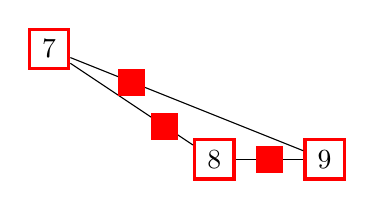
\begin{tikzpicture}[x = 7mm, y=7mm]
%	\draw (-1,-1) rectangle (8,8);
	\tikzstyle{Square} = [
		draw = red, 
		very thick,
		rectangle,
		minimum size = 5 mm
	]
	\tikzstyle{Synth} = [
		draw = red, 
		fill = red,
		very thick,
		rectangle,
		minimum size = 3mm
	]
	\tikzstyle{Circle} = [
		draw = blue, 
		circle,
	]
	\tikzstyle{CircleFill} = [
		draw = blue,
		fill = blue, 
		circle,
	]
	\node [Square] (7) at (0,2) {7};
	\node [Square] (8) at (3,0) {8};
	\node [Square] (9) at (5,0) {9};

	\draw (7) -- (8);
	\draw (7) -- (9);
	\draw (8) -- (9);
	
	\node [Synth] () at ($0.3*(7) + 0.7*(8)$) {};
	\node [Synth] () at ($0.7*(7) + 0.3*(9)$) {};
	\node [Synth] () at ($0.5*(8) + 0.5*(9)$) {};


\end{tikzpicture}
\end{center}

One challenge with SMOTE is that it is only useful for datasets with continuous numerical data, and our data is almost all categorical.  What is between ``car'' and ``school bus,'' or between ``parking lot'' and ``highway''?  SMOTE has a variant, SMOTE-NC (Nominal and Continuous) that can handle datasets with some nominal (categorical) features, but most of the features need to be continuous; thus, we will not be able to use SMOTE or similar techniques for our work.  

%%% Original stuff in Prospectus

Especially if we're doing fatalities, we have a terribly imbalanced data set.  Ideally we'd like to have an equal number of fatal and nonfatal crashes to plug into our ML algorithm, but we have about 0.47\% fatal and 99.53\% nonfatal.  

One solution is to randomly choose 681 nonfatal crashes to compare with our 681 fatal crashes, but that leaves behind a LOT of information.  

Many of the papers I've read use SMOTE, which balances the data set by creating synthetic elements for the minority set (fatal crashes).  It picks an element of the minority set, $a$, and picks one of its nearest neighbors, $b$, and creates a new synthetic element $c$.  For each data category, $D_i$, in which they differ, SMOTE chooses $D_i(c)$ to be between $D_i(a)$ and $D_i(b)$.  It randomly chooses a random number $r \in [0,1]$, and makes $D_i(c) = D_i(a) + r(D_i(a) - D_i(b))$.  

I get how that works for continuous variables.  I get that it would work if $D_i(a)$ and $D_i(b)$ weren't very different.  

How would that work for boolean variables?  SMOTE would choose nearest neighbors $a$ and $b$ that agree on most variables, but for values of $i$ where $D_i(a)=0$ and $D_i(b)=1$, it would randomly choose $D_i(c) \in \{0,1\}$.  There is no {\it between} for boolean variables.  It doesn't seem to me that it would work as well.  

Original SMOTE only works with continuous variables.  There is something called SMOTE-NC that handles continuous and categorical, but it has to have some continuous variables to work on.  

\begin{quote}
Unlike SMOTE, SMOTE-NC for dataset containing numerical and categorical features. However, it is not designed to work with only categorical features.
\end{quote}

\url{https://imbalanced-learn.org/dev/references/generated/imblearn.over_sampling.SMOTENC.html}

Since we have $\approx 200$ times as many nonfatal crashes as fatal crashes, to balance the data set with SMOTE, we would have to make two hundred synthetic elements for each fatal crash.  It seems to me that we would be making a mess of our data set.  
		


%%%
\subsection{Flavors of SMOTE}
\index{SMOTE Flavors}

SMOTE, or Synthetic Minority Oversampling TEchnique, 			\cite{CHAWLA_2002}
 creates extra samples of the minority class, but rather than making exact copies, it finds two similar samples and creates more samples ``between'' them, with feature values between the values of the two samples.  SMOTE only works for continuous features, not for categorical features.  Almost all of my features are categorical.  
 
 I got this list of flavors of SMOTE from a 2021 review by Mahmudah.
			\cite{MAHMUDAH_2021}  I've investigated some of them and given some flesh to some parts of this skeleton.
 
 		\begin{itemize}
			\item SMOTE:  Synthetic Minority Oversampling TEchnique 
			\cite{CHAWLA_2002}
			
			Uses $k$-nearest neighbors to find two close positive (minority) samples, and creates a synthetic sample between them.  Works on continuous data, not on categorical or binary data.  
			
			\item ADASYN:  ADAptive SYNthetic sampling approach for imbalanced learning.  
			\cite{MAHMUDAH_2021}
			
			Creates synthetic samples based on the level of difficulty in learning the samples of the minority class.  A positive samples is ``difficult'' if it has more negative samples as its nearest neighbors.  The more difficult a sample is, the more synthetic copies of that sample ADASYN creates.  
			
			\item Borderline SMOTE
			\cite{MAHMUDAH_2021}
			
			Generates synthetic positive samples along the border between the positive and negative classes.  Brad's Question:  This assumes you know where the border is.  I suppose you could do it iteratively.  
			
			\item Safe-level SMOTE
			\cite{MAHMUDAH_2021}

			When SMOTE finds the nearest positive-class neighbors of a positive sample, it ignores the negative (majority-class) neighbors.  [I think this is what it means:]  Creating synthetic positive-class samples in a neighborhood with lots of negative samples just makes more of a mess, so this is not considered a ``safe'' place to make synthetic samples.  Safe-level SMOTE creates synthetic positive samples only in majority-positive neighborhoods.  
			
			\item Relocating-safe-level SMOTE (RSLS)
			\cite{MAHMUDAH_2021}
			
			Avoids creating synthetic positive samples near negative samples.  
			
			\item Density-based SMOTE (DBSMOTE)
			\cite{MAHMUDAH_2021}

			Integration of DBSCAN and SMOTE.   DBSCAN, Density-Based Spatial Clustering of Application with Noise, discovers clusters with an arbitrary shape (?)  DGSMOTE creates synthetic samples at the pseudo-centroids of the clusters of positive samples.  
			
			\item Adaptive Neighbor SMOTE (ANS)
			\cite{MAHMUDAH_2021}

			Focuses not on -where- to generate synthetic samples, but on -how many- samples to generate in a particular neighborhood. 

			\item D2GAN 

This 2020 article by Zhai \cite{ZHAI_2020_D2GAN} builds on the Dual Discriminator Generative Adversarial Nets (D2GAN) paper from 2017 by Nguyen \cite{NGUYEN_2017}.  They want to do better oversampling, comparing D2GAN with SMOTE.  I don't understand what this is, but they say SMOTE has three drawbacks:

\begin{enumerate}
	\item Ignores the probability distribution of minority class samples.
	\item Synthetic examples lack diversity.
	\item Interating SMOTE many times will give synthetic samples with significant overlap.
\end{enumerate}

This 2022 article by Zhai \cite{ZHAI_2022} slightly modifies Zhai's claims against SMOTE.

\begin{enumerate}
	\item Does not extend the training field of positive samples.
	\item Synthetic examples lack diversity.
	\item Does not accurately approximate the probability distribution of minority class samples.
\end{enumerate}

The authors propose two new methods of diversity oversampling by generative models, one based on ``extreme machine learning autoencoder,'' and the other based on generative adversarial networks (GAN).  

			
		\end{itemize}
		
%%%
\subsection{Oversampling Image Data}
\index{Oversampling Image Data}

Extracting knowledge from a database of tabular numerical or categorical data is difficult, but a database of images is a challenge of a different magnitude.  An imbalanced labeled image dataset for crash prediction modeling might be a thousand images taken ten seconds before a crash and a million images taken ten seconds before ... nothing happened.  Deep neural networks (DNN) and (deep) convolutional neural networks (DCNN and CNN) are common methods for image data.  \cite{NIPS2014_5ca3e9b1} introduced Generative Adversarial Networks, which can be used to generate synthetic samples to balance the dataset.  Given the power of the tools for image recognition, many researchers make non-image data look (to the computer) like images to take advantage of the tools.  



%%%
\subsection{Train/Test Split}
\index{Train/Test Split}

The application in Sharififar's 2019 article \cite{SHARIFIFAR_2019}  is digital mapping of farmland, categorizing areas by soil type.  Some soil types are rare but significant.  This is the first article I've seen that, at the beginning, says that making sure each minority class appears in appropriate distribution in the validation and test sets is an important challenge.  They explicitly say that they split 30\% for the validation set by taking 30\% of each class.

%%%
\subsection{Feature Selection}
\index{Feature Selection}

This 2012 article by Tan \cite{TAN_2012} introduces a feature selection model specifically for imbalanced data sets.  I haven't dug in yet.  




%%%%%
\section{Bagging and Boosting}

%%%
\subsubsection{Bagging}
\index{Bagging}

``Bagging'' is short for Bootstrapped Aggregating, a variation on random undersampling. \cite{BRIEMAN_1996}  In general, bagging takes many random subsets (with replacement) of the samples, run the classifier on each subset, then aggregate the results.  In imbalanced data applications, each subset of the samples is all of the $n$ minority samples and $n$ randomly chosen majority samples.  

Balanced Random Forest [need citation] is a form of bagging.  

In our example, bagging would make a subset of the data with the three minority-class samples (\#7, 8, and 9), and three randomly chosen from the majority-class samples, run the classifier; repeat some number of times.  Use an ensemble classifier to merge the results.  

\begin{center}
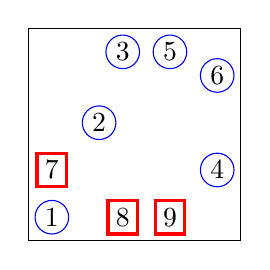
\begin{tikzpicture}[x = 3mm, y=3mm]
	\draw (-1,-1) rectangle (8,8);
	\tikzstyle{Square} = [
		draw = red, 
		very thick,
		rectangle,
		inner sep = 1mm,
		minimum size = 2 mm
	]
	\tikzstyle{SquareFill} = [
		draw = red, 
		fill = red,
		very thick,
		rectangle,
	]
	\tikzstyle{Circle} = [
		draw = blue, 
		circle,		
		inner sep = 0.5mm,
	]
	\tikzstyle{CircleFill} = [
		draw = blue,
		fill = blue, 
		circle,
	]
	\node [Circle] (1) at (0,0) {1};
	\node [Circle] (2) at (2,4) {2};
	\node [Circle] (3) at (3,7) {3};
	\node [Circle] (4) at (7,2) {4};
	\node [Circle] (5) at (5,7) {5};
	\node [Circle] (6) at (7,6) {6};
	\node [Square] (7) at (0,2) {7};
	\node [Square] (8) at (3,0) {8};
	\node [Square] (9) at (5,0) {9};

\end{tikzpicture}
\end{center}

\

Lack (2021)  used bagging in predicting crashes for trucks and finding ways to improve truck safety.  \cite{LACK2021106105}

Shi (2021) developed a
hierarchical over-sampling bagging method based on Grey Wolf Optimizer (GWO) algorithm and Synthetic Minority Over-sampling Technique (SMOTE)
to study lane changing for autonomous vehicles.  The data was severely imbalanced because lane changing is rare compared with lane keeping.  \cite{SHI2021103414}

Chen (2022) used bagging for ride-hailing demand prediction.  \cite{CHEN2022103709} 



%%%
\subsubsection{Boosting}
\index{Boosting}

Boosting is an iterative method that runs the classifier multiple times.  At the end of each iteration, it determines which samples would be misclassified under the current model.  In the next iteration, the classifier gives higher weight to the misclassified samples, improving the model on marginal cases.  While boosting is not just for imbalanced data, the challenge in imbalanced data is that the minority class samples get misclassified, so boosting would help.  A popular implementation is AdaBoost, introduced by \cite{FREUND1997119}.


Haule (2021) used boosting in studying the effects of ramp metering on traffic safety.  \cite{HAULE2021106181}


\begin{itemize}
	\item Boosting and Bagging 
	\cite{BATISTA_2004} 
	\cite{CHABBOUH_2019} 
	\cite{DABLAIN_2021} 
	\cite{MAHMUDAH_2021} 
	\cite{SHARIFIFAR_2019}
\end{itemize}


%%%%%
\section{Lit Review:  Medium.com {\it Towards Data Science} Articles}

These aren't exactly peer reviewed, but they're current.  

Soleymani (4/1/22) says that class weights are more effective than SMOTE, and gives an example of why SMOTE doesn't do what you think it should.   
\cite{Soleymani_TDS_04_01_2022}

Raj (9/5/19) is a brief article that introduces what an imbalanced data set is, and resampling, including na\"ive oversampling, undersampling, and SMOTE.  
\cite{Raj_TDS_09_05_19}

Soni (10/9/20) introduces Balanced Random Forest, with code, in addition to undersampling and oversampling.  Balanced Random Sampling is, I think, a form of bagging.  You take a bootstrap sample of the minority class and the same number of elements from the majority class, and run random forest; then aggregate the results.  
\cite{Soni_TDS_10_09_20}

Brownlee isn't in TDS, but gives an easy introduction to ROC curves.  
\cite{Brownlee_TDS_11_26_14}
Also gives good references in \cite{Brownlee_TDS_08_19_15}.

Stewart also mentions Tomek Links.  
\cite{Stewart_TDS_07_01_22}

Bordia reviews variants of SMOTE, including SMOTE\_NC, which works with datasets with some (but not all) categorical data and some continuous data.  NC is for Nominal and Continuous.  
\cite{Bordia_TDS_02_25_22}

Boyle recommends Random Forests for imbalanced data.  
\cite{Boyle_TDS_02_03_19}

Keras can do random forest classifiers, although you may need to make it yourself.  \url{https://keras.io/examples/structured_data/deep_neural_decision_forests/}

How to do an ROC curve and find AUC for Keras and sklearn: \url{https://medium.com/hackernoon/simple-guide-on-how-to-generate-roc-plot-for-keras-classifier-2ecc6c73115a}

Badr includes bagging.  
\cite{Badr_TDS_02_22_19}

Rocca gives many different ideas.  Read this one carefully.  
\cite{Rocca_01_27_19}

Lador gives good examples of when different metrics are useful.  
\cite{Lador_TDS_09_05_17}

Jaitley also recommends Random Forest, Gradient Boosting, and AdaBoost.
\cite{Jaitley_02_01_19}

Ahamed had entirely different recommendations, Ensemble Cross-Validation (CV), Class Weights, and Over-Predicting the class of the minority class, {\it i.e.} setting a lower probability threshold for the minority class.  
\cite{Ahamed_04_15_18}



%%%%%%%%%%
\chapter{Lit Review:  Datasets}

%%%%%
\section{Crash Datasets}
\index{Crash Datasets}


\begin{itemize}
	\item \acrshort{shrp},  Strategic Highway Research Program 2, Naturalistic Driving Study
	
	Federal Department of Transportation
	
	Most cited dataset.  
	
	\item Second Highway Research Program (Data Set)
	
	I have an account.  
	\item Virginia 100-car Database 
	\item Next Generation Simulation, NGSIM Trajectory Data
	https://iswitrs.chp.ca.gov/Reports/jsp/index.jsp
	\item NASS-CDS:  National Automotive Sampling System – Crashworthiness Data System
	\item Canada's National Collision Database
	\item Michigan Safety Pilot
	\item Roadway Information Database (RID)
	\item Shanghai Naturalistic Driving Study	
	\item California Statewide Integrated Traffic Records System (SWITRS)
	
	Apparently anyone can get an account?
	
	\url{https://iswitrs.chp.ca.gov/Reports/jsp/index.jsp}
	\item Highway Safety Information System
	
	Not updated since 2018?
	
	\url{http://www.hsisinfo.org}
\end{itemize}

%%%%%
\subsection{Jargon to Understand}

From \verb|24_May_2021_Report|:

\begin{itemize}
	\item Naturalistic Driving Data - Data collected from sensors installed in the driver's own car, trying to get as close as possible to the driver's ``natural'' behavior. \index{Naturalistic Driving Data}
	\item Heterogeneity.  I understand vaguely what ``data heterogeneity'' means, but I'm going to watch for the term to see how it's used in the context of these papers.  \index{Heterogeneity}
\end{itemize}

%%%%%
\subsection{IRB, SHRP Database}

Eleven of the papers in {\it Accident Analysis and Prevention} used the Strategic Highway Research Program 2 (SHRP2) Naturalistic Driving Study (NDS), which put sensors in 3400 cars and recorded five million trips, including crashes.  To get ``Qualified Researcher Status'' with ``full access to data that has been made available through the SHRP 2 NDS Data Access Website,'' I had to submit a certificate of training on research with human subjects.  I did the training through the UL Institutional Review Board (IRB). I now have access.  

%%%%%
\subsection{NGSIM Database}

Three papers use the Next Generation Simulation dataset from the US Dept of Transportation, and it's available for download with no restrictions.  




%%%%%
\section{Datasets with Imbalanced Data}

%%%
\subsection{Datasets, Annotated}

%%%%%
\subsection{Articles using These Datasets}

Zheng 2021 \cite{ZHENG_2021}

\begin{itemize}
	\item Oversampling, undersampling, and hybrid methods use random sampling ratios.  [What?  How?  I thought the user set the sampling ratios.]
	\item This paper proposes three algorithms to automatically set the sampling ratios using genetic algorithms.  	
	\item Used fourteen datasets, some of which may be useful benchmark datasets.
\end{itemize}

Wang 2021 \cite{WANG_2021}

\begin{itemize}
	\item Uses seven benchmark imbalanced datasets from the UCI machine learning repository
	\item Implicit regularization for dynamic ensemble selection of classifiers.
\end{itemize}

%%%%%
\subsection{Database Repositories}

UCI Machine Learning Repository

\url{https://archive.ics.uci.edu/ml/about.html}



%%%%%%%%%%
\chapter{Lit Review:  Seminal and Interesting Papers}

%%%%
\section{Seminal Papers}

\begin{itemize}
	\item Lin \cite{LIN_2020} introduced Focal Loss in 2017.  The 2017 versions of this article are only available through Inter Library Loan, because the UL Library apparently doesn't subscribe to IEEE, and the version I found was from 2020.  
 
\end{itemize}
%%%%%
\section{Review Papers}

%%%
\subsection{Chawla}
Chawla \cite{CHAWLA_2004} gives an overview of the state of the field in 2004.

\begin{itemize}
	\item Data Methods
	\begin{itemize}
		\item Random Oversampling with Replacement
		\item Random Oversampling
		\item Directed Oversampling
		
		No new examples are created, but the choice of which ones to replace is informed rather than random.
		\item Directed Undersampling
		\item Oversampling with informed generation of new samples
		\item Combinations of the above
	\end{itemize}
	\item Algorithmic Methods
	\begin{itemize}
		\item Adjusting class costs
		\item Adjusting the probabilistic estimate at the tree leaf (for tree methods)
		\item Recognition-based methods (learning from one class) rather than discrimination-based.
	\end{itemize}
	\item Issues at 2000 Conference
	\begin{itemize}
		\item 
	\end{itemize}
	\item Issues at 2003 ICML Conference
	\begin{itemize}
		\item Probabilistic estimates
		\item Pruning
		\item Threshold adjusting
		\item Cost-matrix adjusting.
	\end{itemize}
	\item Interesting Topics at 2003 ICML Conference
	\begin{itemize}
		\item Selective sampling based on query learning (Abe)
	\end{itemize}
	\item Overlapping Problems
	\begin{itemize}
		\item Class Imbalance
		\item Small Disjunct Problem (?)
		\item Rare Cases
		\item Data Duplication
		\item Overlapping Classes
	\end{itemize}
\end{itemize}

By 2003, the field started to mature.  


%%%
\subsection{Chabbouh 2019}

This article \cite{CHABBOUH_2019} has a nice table classifying existing work in imbalanced classification; however, I think much of the information was old in 2019, particularly C4.5, an early decision tree base classifier that may not be used much anymore.  


%%%
\subsection{Mahmudah 2021}

This article \cite{MAHMUDAH_2021} is really a review of current methods.   They have some datasets, most public benchmark sets, and throw every combination of tools at them. The ``methods'' section is really an overview of current methods.  

Has a section on techniques for feature extraction (feature engineering?) by dimensionality reduction, not particularly related to imbalanced data.  





%%%%%
\section{Examples of Good Writing, Models to Follow}

\begin{itemize}
	\item Elassad 2020 \cite{ELAMRANIABOUELASSAD2020102708} is a good model.	

	\item Paez 2021 \cite{PAEZ2020105666} is not ML, but a solid paper.  The conclusion suggests looking into imbalanced learning.  
	
	\item Soleimani (LSU) 2019 \cite{SOLEIMANI201965} gives a thorough analysis.
\end{itemize}

\subsection{Elassad 2020}

Good model to follow.

\begin{itemize}
	\item In the title and first sentence of the abstract talks about an application, Collision Avoidance Systems, that the paper does not work with directly, which is like what I'm doing with mobile phones.  
	\item Has several glaring mistakes, like crash avoidance systems on the vehicle having access to data from loop detectors, which are embedded under the road.  
	\item Projects into the future, assuming that vehicles will detect the physiological state of the driver.  I do this when I assume that police departments will have access to up-to-date and well-calibrated maps, to personal data from phone companies, and to be able to corollate several pieces of data (from multiple phones) in real time.  
	\item Critique:  Doesn't define terms well.  What is an ``ensemble fusion framework''?  How are ``ensemble'' and ``fusion'' different?  In layman's language, they sound the same.  Uses ``fusion'' to mean both classifier ensembles and data fusion.
	\item Good overview at the end of the Introduction.  
	\item The ML guts of this paper are trying different combinations of classifiers for an ensemble method.  The guts of my paper will be different combinations of imbalanced data techniques.
	\item Only uses two imbalanced data techniques:  Class weights and SMOTE.
	\item Algorithms
	\item Table of features
	\item Six points for future research
\end{itemize}



%%%%%%%%%%
\chapter{Dataset}
%%%%%
\section{Overview}

\subsection{Misspellings}

In the `CITY' feature in the data, the name of the city of Shreveport is spelled nineteen different ways.  It's not a problem, though, because it's spelled correctly about 47,000 times and incorrectly only 35 times.  

%%%%%
\section{Properties}

%%%
\subsection{Boolean Nature of our Data}

Most of our data is boolean.  Was alcohol involved?  Did the car leave its lane?  Was there a pedestrian?  We have categorical variables, like type of vehicle which we represent as dummy (boolean) variables.  We have some categories we could represent as numbers (like day of the week), and we could impose an order, (Monday comes before Tuesday), but the order isn't relevant in predicting injuries or fatalities, (Neither increases or decreases as the days ``progress.''), so we should represent them as categories, in dummy variables.  


%%%
\subsection{Top Twenty Features that Correlate with Fatality}

Last column is the {\it balanced f1} score.

\

\begin{tabular}{llll}
\verb|DR_COND_CD2| & I & DRUG USE - IMPAIRED & 0.33 \cr
\verb|SEC_CONTRIB_FAC_CD| & L & CONDITION OF PEDESTRIAN & 0.32 \cr
\verb|PRI_CONTRIB_FAC_CD| & L & CONDITION OF PEDESTRIAN  & 0.25 \cr
\verb|PRI_CONTRIB_FAC_CD| & M & PEDESTRIAN ACTIONS & 0.20 \cr 
\verb|VEH_TYPE_CD1| & G & OFF-ROAD VEHICLE & 0.18 \cr
\verb|M_HARM_EV_CD1| & B & FIRE/EXPLOSION  & 0.17 \cr
\verb|DR_COND_CD2| & F & APPARENTLY ASLEEP/BLACKOUT & 0.17 \cr
\verb|CRASH_TYPE| & C &  [Unknown] & 0.17 \cr
\verb|SEC_CONTRIB_FAC_CD| & M & PEDESTRIAN ACTIONS & 0.16  \cr 
\verb|M_HARM_EV_CD1| & O & PEDESTRIAN & 0.15 \cr
\verb|VEH_COND_CD| & E & ALL LIGHTS OUT & 0.15 \cr
\verb|F_HARM_EV_CD1| & O & PEDESTRIAN & 0.15 \cr
\verb|M_HARM_EV_CD1| & F & FELL/JUMPED FROM MOTOR VEHICLE & 0.15 \cr
\verb|F_HARM_EV_CD1| & F & FELL/JUMPED FROM MOTOR VEHICLE & 0.14 \cr
\verb|PEDESTRIAN| &&& 0.13 \cr
\verb|VEH_TYPE_CD1| & E & MOTORCYCLE & 0.13 \cr
\verb|DR_COND_CD2| & G & DRINKING ALCOHOL - IMPAIRED & 0.13 \cr
\verb|CRASH_TYPE| & A &  [Unknown] & 0.13 \cr
\verb|MOVEMENT_REASON_2| & G & VEHICLE OUT OF CONTROL, PASSING & 0.12 \cr
\end{tabular}

%%%%%
\section{Thoughts on our Data Set:  Trees}

I suspect that a decision tree is the only realistic way to make a predict model for any aspect of crash data.  If a pedestrian is involved, or it's a rural area, or alcohol is involved, the dynamics of the problem change.  That there could be some linear (or nonlinear) function of all of the variables to fatality or injury is not reasonable to hope.  If we think of it not as one big problem but as lots of little problems, like ``What factors predict a fatality/injury in a crash involving a pedestrian in a rural area at night?'' and, ``What factors predict a fatality/injury in a crash where alcohol is involved at rush hour in an urban area?'',  we'll have much more likelihood of success.  


%%%%%
\section{Times}

From the \verb|Brads_Report_11_01_21|

%%%
\subsection{New Features}
Interesting features I didn't have before:

\begin{itemize}
	\item \verb|AMBULANCE| $\in \{0,1\}$
	\item \verb|CRASH_TIME|
	\item \verb|TIME_POLICE_NOTE|
	\item \verb|TIME_POLICE_ARR|
	\item \verb|TIME_AMB_CALLED|
	\item \verb|TIME_AMB_ARR|
\end{itemize}

In the 828,248 records, 167,662 (20.2\%) have \verb|AMBULANCE|==1.

\subsection{Dirty Data}

In many of the records, one of the times could be 0, which could indicate midnight, but more likely indicates missing data.  Lots of the records mix up AM and PM.  Some of them have the police or ambulance called before the crash time.  In some of them, the ambulance isn't called until more than half an hour after the crash time, which could be real, but more likely a data entry error.  Adding to the messiness is that some of the crashes roll over midnight.  

There may be ways to fix some of those records, but for now I'll thrown them out.  I threw out 47,640 records (28\%), leaving 120,002 records.  

\subsection{Strange Data}

The \verb|CRASH_TIME| feature is in the format ``1/1/01 HH:MM:SS,'' but the second are either ``00'' or ``39.''  I don't know why.  I'm going to ask Malek whether it appears that way in the original Access file.  

\subsection{Ambulance Call within/after 5 min after Crash}

\begin{itemize}
	\item In 64\% of the cases, the ambulance was called within 5 min of the crash.  
	\item In 15\% of the cases, the ambulance was called more than 5 min after the crash and after the police arrived.  Those 18,037 are the interesting cases.  
\end{itemize}

\subsection{Hospitalized}

Of the 120,022 clean records where an ambulance was called, 43,902 (37\%) had no one hospitalized, so while the ambulance crew may have applied minor first aid, it wasn't an emergency.  






%%%%%%%%%%
\chapter{Methods and Experimental Results To Date}
\input{Scikit-Learn}

%%%%%
\section{Focal Loss and Tomek}

Working with our crash database, with the cleaning and organizing in which I had it in February 2022, I tried different values for $\gamma_1$ and $\gamma_2$ with and without Tomek Links cleaning.  

Tomek Links is a method for cleaning a noisy dataset for binary classification.  A {\it Tomek Link} is a pair of samples, one from the positive and one from the negative class, that are each others' closest neighbors.  The idea is that one of them is noise, or that having these two interferes in making a good classification, that you want the classes to cluster.  In a balanced dataset you eliminate both of them from the training set.  In an imbalanced dataset, you eliminate the element from the majority class.  

From my weekly report 2/21/22:

\begin{itemize}
	\item Unfortunately, $p$ means two different things below.  
	\begin{itemize}
		\item $p_i$ is the probability returned by the model that each sample belongs to the positive set.
		\item $p$ is a hyperparameter, ideally the proportion of the negative to positives samples, to use $\alpha = p/(p+1)$ in the Focal Loss function, to create the class weights that have the same effect as random oversampling.  In our dataset, $p=88.8$.  (No, I'm not kidding.)
	\end{itemize}
	\item All runs without Tomek used the same training and test sets
	\item All runs with Tomek used the same training and test sets
	\item The two test/train splits used the same random sampling seed, so they should be the same sets.
\end{itemize}


\begin{align*}
	\text{Focal Loss} &= \sum_{i=1}^n \alpha (1 - p_i) ^{\gamma_1} y_i \log (p_i) + (1 - \alpha) p_i^{\gamma_2} (1 - y_i)  \log (1 - p_i) \cr
	 &= \sum_{y_i=1} \alpha (1 - p_i) ^{\gamma_1} \log (p_i) + \sum_{y_i=0} (1 - \alpha) p_i^{\gamma_2}   \log (1 - p_i) \cr
	\end{align*}

%%%
\subsection{Different Values of $p$ with $\gamma_1=0$, $\gamma_2=0$}

\begin{tabular}{rrrrrrrl}
	& Tomek? & $p$ & $\gamma_1$ & $\gamma_2$ & TN/FN & FP/TP & Comments\cr\hline
	& No & 1 & 0 & 0 &  573308  &  0 \cr
	&&&&&  6466  &  0 \cr \hline
	&No & 20&0&0&  562182  &  11126 \cr
	 &&&&&  5850  &  616 \cr\hline
	& No & 88.8 & 0 & 0 &  428929  &  144379 & This is the natural $p$ \cr
 	&&&&& 3105  &  3361 & for our dataset. \cr	\hline
	& No & 100 & 0 & 0 &  411813  &  161495 \cr
	 &&&&&  2737  &  3729 \cr\hline
	 & No  & 200 & 0 & 0 &  287151  &  286157 \cr
	 &&&&&  1464  &  5002 \cr\hline
\end{tabular}

%%%
\subsection{Fixed $p=88.8$, Different values of $\gamma_1$ and $\gamma_2$}

\begin{tabular}{rrrrrrrl}
	& Tomek? & $p$ & $\gamma_1$ & $\gamma_2$ & TN/FN & FP/TP & Comments\cr\hline
	& No & 88.8 & 0.0 & 0.0 &  428929  &  144379 & This is the natural $p$ \cr
 	&&&&& 3105  &  3361 & for our dataset. \cr	\hline
	 & No & 88.8 & 0.5 & 0.5 &  399870  &  173438 \cr
	 &&&&&  2685  &  3781 \cr\hline
	 & No & 88.8 & 1.0 & 1.0 &  420343  &  152965 \cr
 	&&&&&  3092  &  3374 \cr\hline
 	& No & 88.8 & 2.0 & 2.0 &  433805  &  139503 \cr
 	&&&&&  3213  &  3253 \cr\hline
	 & No & 88.8 & 5.0 & 5.0 &  445445  &  127863 \cr
	 &&&&&  3519  &  2947 \cr\hline
	  & No & 88.8 & 0.0 & 2.0 &  337148  &  236160 \cr
	 &&&&&  2092  &  4374 \cr\hline
	  & No & 88.8 & 0.5 & 0 &  460148  &  113160 \cr
	 &&&&&  3520  &  2946 \cr\hline
	  & No & 88.8 & 1.0 & 0.0 &  391820  &  181488 \cr
	 &&&&&  2596  &  3870 \cr\hline
	 & No & 88.8 & 2.0 & 0.0 &  527871  &  45437 \cr
	 &&&&&  4877  &  1589 \cr\hline
 \end{tabular}
 
 %%%
 \subsection{Tomek}
 
 Tomek took out 760 negative samples, bringing $p$ down to $88.66$.

\
 
 \begin{tabular}{rrrrrrrl}
	& Tomek? & $p$ & $\gamma_1$ & $\gamma_2$ & TN/FN & FP/TP & Comments\cr\hline
	& No & 88.8 & 0.0 & 0.0 &  428929  &  144379 &  \cr
 	&&&&& 3105  &  3361 &  \cr	\hline
	& Yes & 88.8 & 0.0 & 0.0 &  387313  &  185995 & FN goes up 29\% \cr
	 &&&&&  2504  &  3962 & TP goes up 18\% \cr\hline
	& Yes & 88.66  & 0.0 & 0.0 &  387313  &  185995 \cr
	 &&&&&  2504  &  3962 \cr\hline
 \end{tabular}

%%%%%
\subsection{Discussion}

\begin{itemize}
	\item The different values of $p$, $\gamma_1$, and $\gamma_2$, and Tomek, give us different tradeoffs between false positives and false negatives, but no combination gives us fewer of both.  
	\item It would be challenging to argue that one set of hyperparameters is ``better'' than another. 
	\item I suspect that there just isn't enough of a pattern in this crash data to give us much confidence.  
	\item I need to also work on other datasets that either might give clearer results, or will show me that all results are this fuzzy and I need to learn how to deal with it.  
\end{itemize}



%%%%%
\section{Feature Engineering}

%%%
\subsection{Time of Day}

Time of day is a continuous variable, but the correlation between time of day and [anything] is nonlinear.  We could do some kind of data transformation, perhaps taking the ratio of the number of accidents to the typical traffic density at that time of day, but the typical car trip at 3 am on a Wednesday may be different in character than a car trip at 7 am on a Saturday, even if the traffic volumes are similar.  Perhaps we should have boolean variables:

\begin{itemize}
	\item Morning rush hour
	\item Mid-day
	\item Afternoon rush hour
	\item Evening
	\item Late night
\end{itemize}

and another variable, {\tt Weekend}.

%%%
\subsection{Number of Fatalities/Injuries}

The number of fatalities or injuries is a function of how many people were in each vehicle, which (a) we don't know and (b) probably isn't correlated to any other data we have.  Fatality and injury should be  boolean variables, that there was a fatality or there was an injury, rather than a count of the number of fatalities or injuries.  

%%%
\subsection{Day of Week}

\begin{figure}[h!]
\centering
\begin{minipage}{.27\textwidth}
  \centering
  \includegraphics[scale=0.32]{../../../Fall_2021/699/Keras//12_04_21_Images/n_Accidents_DAY_OF_WK.png}
  \caption{Number of Crashes, by Day of Week}
  \label{fig:test1}
\end{minipage}%
\begin{minipage}{0.05\textwidth}
\
\end{minipage}
\begin{minipage}{.27\textwidth}
  \centering
  \includegraphics[scale=0.32]{../../../Fall_2021/699/Keras//12_04_21_Images/n_Severe_DAY_OF_WK.png}
  \caption{Number of Severe Injury Crashes, by Day of Week}
  \label{fig:test2}
\end{minipage}
\begin{minipage}{0.05\textwidth}
\
\end{minipage}
\begin{minipage}{.27\textwidth}
  \centering
  \includegraphics[scale=0.32]{../../../Fall_2021/699/Keras//12_04_21_Images/p_Severe_DAY_OF_WK.png}
  \caption{Percentage of Crashes with Severe Injury, by Day of Week}
  \label{fig:test2}
\end{minipage}
\end{figure}


My understanding is that, for feature engineering, we don't care that there are more crashes on Friday than other weekdays, since the proportion of crashes that require an ambulance are the same.  Saturday and Sunday, though, are different.

I made a feature, \verb|Weekday_SA_SU|:

\begin{center}
\begin{tabular}{rl}
	0 & MO, TU, WE, TR, FR\cr
	1 & SA \cr
	2 & SU \cr
\end{tabular}
\end{center}

\newpage
%%%
\subsection{Time of Day}

\begin{figure}[h!]
\centering
\begin{minipage}{.45\textwidth}
  \centering
  \includegraphics[scale=0.5]{../../../Fall_2021/699/Keras/12_04_21_Images/n_Weekday_by_Hour.png}
  \caption{Number of Weekday Crashes, by Hour}
  \label{fig:test1}
\end{minipage}%
\begin{minipage}{0.08\textwidth}
\
\end{minipage}
\begin{minipage}{.45\textwidth}
  \centering
  \includegraphics[scale=0.5]{../../../Fall_2021/699/Keras/12_04_21_Images/p_Weekday_by_Hour}
  \caption{Percentage of Weekday Crashes with Severe Injury, by Hour}
  \label{fig:test2}
\end{minipage}
\end{figure}

I note with interest that, at 7am, the number of crashes spikes, but the percentage of severe injury crashes does not change significantly.  I created a \verb|Rush_Hour| feature, but I don't know if it will be of any use.  


The spike of percentage of crashes at 1am is just noise, because of the small number of crashes at that time.    


\

The types of roads on which crashes occurs varies widely by time of day.  I don't know what to do with that.  


\begin{figure}[h!]
\centering
\begin{minipage}{.45\textwidth}
  \centering
  \includegraphics[scale=0.5]{../../../Fall_2021/699/Keras/12_04_21_Images/Interstate_Crash_Percentage_by_Hour.png}
  \caption{Percentage of Crashes on Interstates, by Hour}
  \label{fig:test1}
\end{minipage}%
\begin{minipage}{0.08\textwidth}
\
\end{minipage}
\begin{minipage}{.45\textwidth}
  \centering
  \includegraphics[scale=0.5]{../../../Fall_2021/699/Keras/12_04_21_Images/City_Street_Crash_Percentage_by_Hour}
  \caption{Percentage of Crashes on City Streets, by Hour}
  \label{fig:test2}
\end{minipage}
\end{figure}


I made a feature, \verb|Time_of_Day|, grouping together times with similar percentages of crashes having severe injuries:

\begin{center}
\begin{tabular}{rl}
	0 & Midnight - 3:00 am\cr
	1 & 3:00 am - 5:00 am\cr
	2 & 5:00 am - 7:00 am \cr
	3 & 7:00 am - 5:00 pm \cr
	4 & 5:00 pm - Midnight \cr
\end{tabular}
\end{center}


%%%%%%%%%%%%%%%%%%
\subsection{Location}
	Location seems like it would be very important.  One proxy we have is the parish and the road name.  I've made a new feature, concatenating the parish and the road name.  Each unique value in that feature will become a category, yielding a new feature in the dummy (one-hot encoding) dataframe that we will use for training.
	
	There are 6.150 unique values, but most of them have few records.  How many records do you need to make a useful correlation, and how many categories will overload the training?
	
	Having a minimum of 1000 records per category gives me 142 categories plus 492,367 records in ``Other''; a minimum of 100 records gives me 1103 categories plus 221,644 records in ``Other.''  A minimum of 10 records gives me 2,534 categories and 171,802 in ``Other.''  Note that 161,454 are in ``Other'' because of missing data.


%%%%%
\subsection{Parish/Road Names}

\begin{itemize}
	\item We have 161,454 records with "0" for the \verb|PRI_ROAD_NAME|.  There's nothing we can do to recover those.  
	\item  We have 26,289 different values for \verb|PRI_ROAD_NAME|.  
	\item We have even more if we combine those with the, sometimes multiple, \verb|PRI_ROAD_TYPE|, like St, Ave, and Blvd.
 \item In a few instances, roads with the same \verb|PRI_ROAD_NAME| and different \verb|PRI_ROAD_TYPE| are different roads, but usually within the same parish they're the same.  A noteable exception is North St and North Blvd in Baton Rouge.
 \item For long roads, like interstates and some state highways, crash outcomes may differ based on which section of road you're on.
 \item To Do:
 	\begin{itemize}
		\item Combine  \verb|PARISH_CD| and \verb|PRI_ROAD_NAME| into a new feature,  \verb|PARISH_CD_and_PRI_ROAD_NAME|.
		\item Ignore the \verb|PRI_ROAD_TYPE|
		\item Keep the instances of  \verb|PARISH_CD_and_PRI_ROAD_NAME| that have more than 1000 crashes.  
		\item Change all of the others to "Other".
	\end{itemize}
 \item Results:
 	\begin{itemize}
		\item This leaves us with 142 different names with 335,880 crashes, plus ``Other'' with 492,367 crashes.  
		\item \verb|PRI_ROAD_NAME| = "AIRLINE" appears (with at least 1000 crashes) in 11 parishes, with 51,399 crashes.
	\end{itemize}
   \end{itemize}






%%%%%%%%%%
\chapter{Research Plan}
%%%%%
\section{Goals}

\subsection{CRSS Data Set}

\acrfull{crss} \cite {CRSS}

\begin{itemize}
	\item Answer question about whether binning or imputing should come first
	\item Some of the binning is not consistent; make a clear rationale for binning and apply it
	\item Finish preparing the data
	\item Apply imbalanced data techniques, testing individually and in combination
	\item Analyze results
\end{itemize}

\subsection{Paper for {\it Transportation Research Part C:  Emerging Technologies}}

\begin{itemize}
	\item Reread papers from this journal that are models of good writing
	\item Read and reread the submission policies
	\item Revise paper
	\item Make a list of opportunities for future research
	\item Write and post technical paper
	\item Submit
	\item Get feedback
	\item Respond to feedback
\end{itemize}	

\subsection{Louisiana Data Set}

\begin{itemize}
	\item Select features to match/complement what I did with CRSS data
	\item Clean
	\item Discretize data.  This will be different from what I did with CRSS, because some of the data is continuous
	\item Impute missing values
	\item Apply imbalanced data in a way that matches/complements what I did with the CRSS data
	\item Analyze results
\end{itemize}

\subsection{Write Dissertation}

\begin{itemize}
	\item Review the literature again
	\item Find and review good examples of dissertations
	\item Write
	\item Revise
	\item Repeat
\end{itemize}



%%%%%
\section{Progress}

%%%%%
\section{Steps}



%%%%%
\newpage
\phantomsection
\addcontentsline{toc}{chapter}{Bibliography}
\printbibliography



%%%%%%%%%%%%%%%%
\end{spacing}
\end{document}

%%%%%%%%%%%%
% Useful tools
%%%%%%%%%

\begin{lstlisting}
Put your code here.
\end{lstlisting}

\lstinputlisting[language=python]{source_filename.py}


